\pdfoutput=1
\documentclass[11pt]{amsart}
\usepackage[T1]{fontenc}
\usepackage[utf8]{inputenc}
\usepackage{lmodern}
\usepackage[a4paper,textwidth=15.5cm,textheight=23.5cm,centering]{geometry}
\usepackage{mathtools,amssymb,amsthm}
\usepackage{microtype}
\usepackage{enumitem}
\usepackage{tikz}
\usetikzlibrary{arrows.meta,positioning}
\usepackage{booktabs,tabularx}
\usepackage[unicode,colorlinks=true,linkcolor=blue!45!black,citecolor=blue!45!black,urlcolor=blue!45!black]{hyperref}
\hypersetup{pdftitle={A Rice theorem for stationary states under fixed noise},pdfauthor={Seth Douglas and Nidhal Mghirbi},pdfsubject={Undecidability and stationary states of noisy lattice dynamics}}
\newtheorem{theorem}{Theorem}[section]
\newtheorem{lemma}[theorem]{Lemma}
\newtheorem{proposition}[theorem]{Proposition}
\newtheorem{corollary}[theorem]{Corollary}
\newtheorem{maintheorem}{Theorem}
\renewcommand{\themaintheorem}{\Alph{maintheorem}}
\theoremstyle{definition}
\newtheorem{definition}[theorem]{Definition}
\theoremstyle{remark}
\newtheorem{remark}[theorem]{Remark}
\numberwithin{equation}{section}
\DeclareMathOperator{\Ext}{Ext}
\DeclareMathOperator{\Tr}{Tr}
\DeclareMathOperator{\Cov}{Cov}
\DeclareMathOperator{\supp}{supp}
\newcommand{\Z}{\mathbb Z}
\newcommand{\R}{\mathbb R}
\newcommand{\N}{\mathbb N}
\newcommand{\one}{\mathbf 1}
\newcommand{\eps}{\varepsilon}
\newcommand{\TI}{\mathrm{TI}}
\newcommand{\cK}{\mathcal K}
\newcommand{\cC}{\mathcal C}
\newcommand{\cB}{\mathcal B}
\newcommand{\cD}{\mathcal D}
\newcommand{\cR}{\mathcal R}
\newcommand{\cQ}{\mathcal Q}
\newcommand{\frakc}{\mathfrak c}
\newcommand{\ord}{\mathrm{ord}}
\newcommand{\Br}{\mathrm{Br}}
\setlist[enumerate]{label=\textup{(\roman*)},leftmargin=2em,itemsep=3pt,topsep=4pt}
\setlist[itemize]{leftmargin=1.7em,itemsep=2pt,topsep=4pt}
\allowdisplaybreaks[2]
\setlength{\emergencystretch}{2em}
\raggedbottom
\title[Stationary states under fixed noise]{A Rice theorem for stationary states\\under fixed noise}
\author{Seth Douglas}
\author{Nidhal Mghirbi}
\date{Version 2.0.0, November 2026}
\subjclass[2020]{60K35, 37B15, 03D35, 81P45}
\keywords{Probabilistic cellular automata, stationary states, undecidability, Rice theorem, Bragg order, local quantum channels}
\begin{document}
\begin{abstract}
Which macroscopic questions about a noisy lattice can an algorithm decide from its local rule? We show that already on the line, for deterministic finite-range rules followed by independent uniform replacement at one fixed positive rational rate, every nontrivial property determined by the number of extreme translation-invariant stationary laws, all-law ergodicity, and the existence of a translation-invariant stationary law with nondecaying local covariance is undecidable. A refined theorem retains the numbers of extreme translation-invariant stationary states with nondecaying covariance and with a Bragg atom at some nonzero wavevector. The same holds for circuits of local quantum channels on the line with independent single-qubit depolarization after every layer, and, with uniqueness among all Gibbs measures in place of ergodicity, for Gibbs measures on the square lattice given by positive rational Boltzmann weights. On the line, ergodicity excludes nondecaying covariance, and two or more translation-invariant stationary states force nondecaying covariance and exclude ergodicity, so only four kinds of coarse data can occur. In both line categories, for every $r\ge1$ the cut ``at most $r$ extremes'' is $\Pi^0_2$ and halting-hard, and for every $k\ge2$ the cut ``at least $k$'' is $\Sigma^0_2$ and nonhalting-hard. In dimension seven the same Rice theorem holds for quantum circuits followed by whole-site depolarization, and under a stated published-source condition $C_T$, at another fixed rational rate, these cuts are $\Pi^0_2$-complete and $\Sigma^0_2$-complete in both categories. The scope has a decidable boundary: a classical translation-invariant stationary law attains the noise entropy floor exactly when the deterministic rule is constant.
\end{abstract}
\maketitle
\begin{center}
\small Claude Opus 5.5, GPT-6.1 Sol, GPT-6.2 Sol and GPT-6.2 Astra assisted with this work; the authors take responsibility for every claim.
\end{center}
\begin{center}\small
Archival record: \href{https://doi.org/10.5281/zenodo.24241163}{doi:10.5281/zenodo.24241163}.
\end{center}
\section{Introduction}\label{sec:intro}
Positive noise gives every local transition a positive probability. It does not give an algorithm for deciding which stationary states survive in infinite volume. We study a finite deterministic lattice rule followed, at every site and time, by independent uniform replacement. The local rule is the input; the dimension and replacement rate are fixed throughout the decision problem.

Our main assertion has the Rice form: every nontrivial property of a specified stationary datum is undecidable. Here nontrivial means that the property holds for at least one valid input and fails for another. A translation-invariant stationary law is extreme when it is an extreme point of the convex set of such laws. We count these extreme points with their full cardinality. All-law (quantumly, all-state) ergodicity means local convergence to one stationary law or state from every initial law or state, including spatially noninvariant ones. We use the term all-law ergodicity in both categories.

The classical conclusion can be stated without the construction's machinery.
\begin{maintheorem}\label{thm:core}
For deterministic finite-range rules on $\Z^7$ followed by uniform replacement at one fixed positive rational rate, every nontrivial property determined by the number of extreme translation-invariant stationary laws, all-law ergodicity, and existence of a translation-invariant stationary law with nondecaying local covariance is undecidable.
\end{maintheorem}

The rate is explicit in \eqref{eq:constants}. The alphabet and finite range may vary. The conclusion includes uniqueness of the translation-invariant stationary law, ergodicity, and every nontrivial cardinality condition on the extreme set. The same parameters work for all properties at once.

One might expect every property of the stationary laws to be undecidable. That is false, and the counterexample fixes the scope. We prove that a stationary spatial Shannon entropy density attains the minimum forced by replacement noise exactly when the deterministic local rule is constant. A finite table scan decides this property. Binary reset and noisy identity have the same datum in Theorem~\ref{thm:core}, but opposite entropy-floor verdicts. Thus the datum, rather than the phrase ``stationary property'', identifies the Rice class.

The covariance flag in Theorem~\ref{thm:core} allows mixtures. Two distinct translation-invariant stationary laws already give a mixture with nondecaying covariance, by the variance of spatial averages. Order in an individual extreme state is a more discriminating question. Our stronger theorem retains both the number of ordered extreme states and the number having a Bragg atom at some nonzero wavevector. It holds for classical rules and for finite-depth local quantum circuits with whole-site depolarization. The construction and its two outcomes appear in Figure~\ref{fig:mechanism}.

The proof couples an arbitrary input, the host, to a computable controller built from a Wang tile set, with one shared replacement flag per site. If the tile set does not tile the plane, the controller forgets every initial configuration on a common event whose probability tends to one, and the coupled medium has exactly the host's datum. If it tiles, every coupled medium has one fixed datum with continuum many ordered extreme TI stationary states. That value absorbs every host, so any property that separates it from some input is as hard as halting or nonhalting. The dimension is six for the imported controller plus one direction of independent slices.

\begin{figure}[ht]
\centering
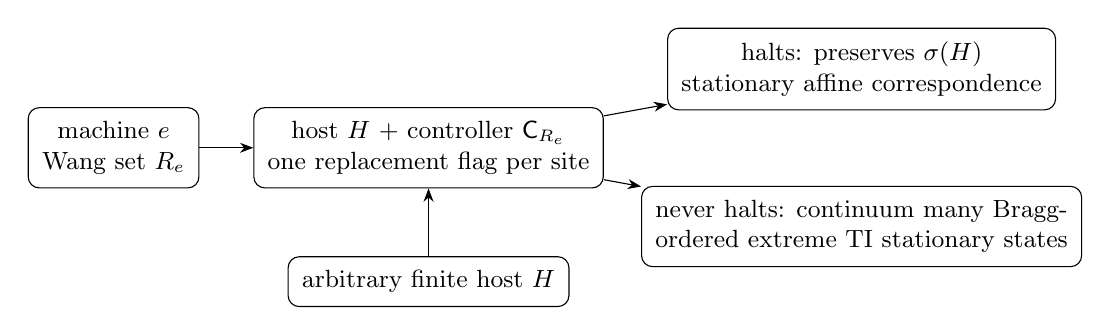
\begin{tikzpicture}[>=Stealth,box/.style={draw,rounded corners,align=center,font=\small,inner sep=5pt}]
\node[box] (e) at (0,0) {machine $e$\\Wang set $R_e$};
\node[box] (j) at (4.0,0) {host $H$ + controller $\mathsf C_{R_e}$\\one replacement flag per site};
\node[box] (h) at (4.0,-1.7) {arbitrary finite host $H$};
\node[box] (d) at (9.5,1) {halts: preserves $\sigma(H)$\\stationary affine correspondence};
\node[box] (l) at (9.5,-1) {never halts: continuum many Bragg-\\ordered extreme TI stationary states};
\draw[->] (e)--(j);\draw[->] (h)--(j);\draw[->] (j)--(d);\draw[->] (j)--(l);
\end{tikzpicture}
\caption{One finite construction separates an arbitrary host datum $\sigma(H)$ (Section~\ref{sec:framework}) from a universal datum. The controller pairs two registers, uses independent slices and swaps registers on alternate sites, which produces a period-two peak at $q_\pi=(\pi,\ldots,\pi)$. Its crystalline states are extreme among TI states; each averages two non-TI periodic stationary states.}\label{fig:mechanism}
\end{figure}

The total phase count also has a precise arithmetical degree. Here a phase means an extreme TI stationary law or state. Under the published-source condition $C_T$ in Section~\ref{sec:completeness}, Theorem~\ref{thm:completeness} makes ``at most $r$ phases'' $\Pi^0_2$-complete for every $r\ge1$ and ``at least $k$ phases'' $\Sigma^0_2$-complete for every $k\ge2$, in both input categories at another single fixed rational rate. A stationary version of host preservation gives one-sided second-level hardness for every nontrivial predicate of $(N,N_{\ord},N_{\Br},L)$ and excludes nontrivial $\Delta^0_2$ members. The total-count cuts are the concrete complete instances; the ordered counts and covariance flag have no arithmetic upper bounds established here.

\subsection{Relation to earlier work}
Rice's theorem concerns nontrivial semantic properties of computably enumerable sets \cite{rice}. Kari established the corresponding theorem for limit sets of one-dimensional cellular automata \cite{kari-rice}; Guillon and Richard refined its fixed-alphabet aspects \cite{guillon-richard}. Delacourt proved Rice theorems for $\mu$-limit sets and generic limit sets \cite{delacourt,delacourt-generic}. Hellouin de Menibus and Sablik, and Delacourt and Hellouin de Menibus, obtained Rice theorems for sets of limit measures from random initial configurations \cite{hellouin-sablik,delacourt-hellouin}. Their dynamics is deterministic. Table~\ref{tab:landscape} places ongoing noise beside these limit constructions.

\begin{table}[ht]
\centering\small
\begin{tabularx}{\textwidth}{@{}>{\raggedright\arraybackslash}p{3.6cm}>{\raggedright\arraybackslash}X>{\raggedright\arraybackslash}X@{}}\toprule
Sources & Object and randomness & Undecidable question\\\midrule
Kari; Delacourt & Deterministic CA limit sets; random initial data for $\mu$-limits & Nontrivial properties of the limit object\\
Hellouin de Menibus--Sablik; Delacourt--Hellouin de Menibus & Limit-measure sets from a Bernoulli initial law & Nontrivial properties of these sets\\
Kurdyumov; Toom; Bu\v{s}i\'c--Mairesse--Marcovici & PCA allowing zero transition probabilities & Ergodicity\\
Marsan--Sablik & Uniform perturbation as noise tends to zero & Stochastic stability\\
Marcovici--Taati & Positive-rate PCA with fixed uniform noise & Stationary Bernoulli existence versus nonexistence\\
Douglas--Mghirbi preprints & Fixed-noise controllers and noise diagrams & Ergodicity and stationary multiplicity\\
This paper & Stationary classical and quantum states at fixed positive noise & Every nontrivial predicate of the stated datum\\\bottomrule
\end{tabularx}
\caption{Undecidability results for cellular automata and PCA, by object and source of randomness.}\label{tab:landscape}
\end{table}

Undecidability of PCA ergodicity goes back to Kurdyumov and Toom \cite{kurdyumov,toom-undecidable,toom-continuous,toom-book,gacs-survey}. Their local rules may have zero transition probabilities. Bu\v{s}i\'c, Mairesse and Marcovici prove that ergodicity of a deterministic one-dimensional CA is equivalent to nilpotency \cite{busic-mairesse-marcovici}, whose undecidability is due to Kari \cite{kari-nilpotency}. Unique ergodicity for deterministic CA is also undecidable \cite{torma}; that temporal notion concerns invariant measures of the deterministic map. It is distinct from uniqueness within the TI stationary set used for our count.

Marsan and Sablik prove undecidability of stochastic stability under uniform perturbations in the zero-noise limit \cite{marsan-sablik}. Marcovici and Taati prove computable inseparability between positive-rate PCA admitting the uniform stationary Bernoulli law and those admitting no stationary Bernoulli law \cite[Theorem~3]{marcovici-taati}. Their construction permits a chosen fixed rational replacement rate. The additional assertion here is the Rice closure over our stationary datum. Work of Toom and G\'acs explains how persistent memory can coexist with positive rates \cite{Toom80,gacs2001}. Marsan, Sablik and T\"orm\"a exhibit a perturbed CA with two ergodicity transitions \cite{marsan-sablik-torma}.

Gu, Weedbrook, Perales and Nielsen formulated a Rice programme for macroscopic ground-state properties of periodic Ising systems and expected it to extend to positive temperature \cite{gu-et-al}. At a fixed positive temperature, Sandhu proved that uniqueness of the Gibbs state is undecidable for a computable family of translation-invariant finite-range interactions on $\Z^2$ \cite{sandhu}; see also \cite{DMthermal}. For quantum ground states, spectral-gap and phase-diagram undecidability were established by Cubitt, P\'erez-Garc\'ia and Wolf and by Bausch, Cubitt and Watson \cite{cubitt-perez-garcia-wolf,bausch-cubitt-watson}. Our quantum dynamics is dissipative and locally implemented. Its hardness is inherited from a classical measure-and-prepare controller. Carrasco-Vargas proved that every nontrivial dynamical property of sofic subshifts on groups with undecidable domino problem is undecidable, and that computable real invariants of SFTs monotone under disjoint unions and products are constant \cite{carrasco-vargas}; our bath invariance plays a role similar to his product monotonicity.

Effective symbolic systems and entropy invariants are treated more broadly by Hochman and by Hochman and Meyerovitch \cite{hochman,hochman-meyerovitch}. Zero-noise limit-measure sets are characterized by Marsan and Sablik \cite{marsan-zero}.

For isolated quantum dynamics, Shiraishi and Matsumoto prove undecidability of thermalization even for one-dimensional shift-invariant nearest-neighbor systems with a fixed product initial state \cite{shiraishi-matsumoto}.

Our earlier preprints prove that ergodicity is undecidable at one fixed rate on $\Z^6$, $\Z^4$ and $\Z^3$, and that a stacked controller on $\Z^7$ has either exactly one invariant measure or a continuum of extreme ones, with no algorithm deciding which \cite[Corollary~3.11]{DMforget}. They also give one noisy automaton with an uncomputable noise diagram \cite{DMdiagram}, and they prove spontaneous magnetization and Gibbs uniqueness undecidable at a fixed positive temperature \cite{DMthermal}. The classical uniqueness, ergodicity and total-count instances of Theorem~\ref{thm:core} therefore already follow from \cite{DMforget}, whose controller theorem we import. The present contribution is the host-preserving construction and its Rice closure, the ordered and Bragg-ordered extreme counts, the long-range-order flag, the quantum category, and the conditional completeness theorem. We did not find a theorem with this stationary-law Rice scope in the literature checked.

\subsection{Reading guide}
Section~\ref{sec:framework} defines the inputs and refined theorem. Section~\ref{sec:controller} states the imported Wang theorem and constructs the crystalline states. Probability readers can proceed to the stationary correspondence in Section~\ref{sec:preservation}; quantum readers will also find its circuit implementation and treatment of entangled inputs there. Section~\ref{sec:rice} completes the halting reduction and invariance arguments. Statistical mechanics readers can read the crystalline amplification together with the entropy boundary in Section~\ref{sec:entropy}. Symbolic-dynamics and computability readers can treat the Wang theorem and the explicitly conditional source interface in Section~\ref{sec:completeness} as black boxes, then follow the totality reduction there and the effective convex geometry in Appendix~\ref{sec:counts}.




\section{Inputs, stationary data and the refined theorem}\label{sec:framework}
\subsection{Two effective input categories}
A classical input consists of a nonempty finite alphabet $\mathsf A$, a finite stencil $\mathcal N\subset\Z^7$, and a deterministic table $F:\mathsf A^{\mathcal N}\to\mathsf A$. One round applies $F$ at every site and then replaces each whole output symbol independently by a uniform symbol with probability $\eps_0$. The flags and replacement values are independent across sites and times. The resulting local transition probabilities are
\[
 p(a\mid u)=(1-\eps_0)\one_{\{a=F(u)\}}+\eps_0/|\mathsf A|.
\]
All entries are positive. Finite alphabets and stencils are unbounded over the input category.

A quantum input has a finite-dimensional site space $\mathbb C^d$ and a finite list of layers of finite-range local completely positive trace-preserving (CPTP) gates. Gates have exact algebraic Choi or Kraus entries and use fresh independent product ancillas. A layer acts on disjoint registers; a finite periodic schedule is permitted when the overall channel $\Phi$ is translation invariant. CPTP validity and overall translation invariance are promises on the presentation. After $\Phi$, every whole site independently undergoes
\[
 \cD_{\eps_0}(X)=(1-\eps_0)X+\eps_0\Tr(X)I_d/d.
\]
Arbitrary initial states, including entangled ones, are allowed. Disjoint sufficiently distant output cones use disjoint circuits and independent environments. A causal channel supplied with globally shared randomness need not have this property and is outside this category.

\subsection{The datum}
Write $\cK(M)$ for the compact convex set of all translation-invariant stationary laws or states of $M$. Translation invariance always means invariance under every spatial translation. In both categories, local convergence means convergence of every finite-region marginal. A state is extreme here precisely when it belongs to $\Ext\cK(M)$.

For real classical or Hermitian quantum local observables $f,g$, write
\[
 \Cov_\omega(f,\tau_xg)=\omega(f\tau_xg)-\omega(f)\omega(\tau_xg).
\]
Let $\ell(\omega)$ mean that some such $f,g$ satisfy
$\limsup_{|x|\to\infty}|\Cov_\omega(f,\tau_xg)|>0$.
For $B_n=\{0,\ldots,n-1\}^7$ and a nonzero wavevector
$q\in(\R/2\pi\Z)^7$, define
\begin{equation}\label{eq:bragg}
 \operatorname{Av}_n^q(f)=\frac1{|B_n|}\sum_{x\in B_n}e^{-iq\cdot x}\tau_xf,
 \qquad b_q(\omega)\iff
 \exists f:\limsup_n\omega\bigl(\operatorname{Av}_n^q(f)^*\operatorname{Av}_n^q(f)\bigr)>0.
\end{equation}
When $b_q(\omega)$ holds we say that $\omega$ has a Bragg atom at $q$. To see the spectral meaning, implement translations in the classical $L^2$ space or the quantum GNS space. For the commuting unitaries $V_i=e^{-iq_i}U_i$, cube averages vanish on every coboundary $v-V_iv$ by telescoping. The closed span of these coboundaries has orthogonal complement the joint fixed space. Contraction and density show that the cube averages converge to its orthogonal projection. The second moment in \eqref{eq:bragg} therefore has a limit equal to the squared norm of the projection of the observable vector.

The refined datum is
\begin{equation}\label{eq:datum}
 \sigma(M)=(N,N_{\ord},N_{\Br},E,L),
\end{equation}
where
\begin{align*}
 N&=|\Ext\cK(M)|,\\
 N_{\ord}&=|\{\omega\in\Ext\cK(M):\ell(\omega)\}|,\\
 N_{\Br}&=|\{\omega\in\Ext\cK(M):\exists q\ne0\ b_q(\omega)\}|.
\end{align*}
Here $E$ means that a unique stationary state among all states attracts every initial state locally; $L$ means $\exists\omega\in\cK(M):\ell(\omega)$. The cardinalities are full cardinalities. In particular $N_{\Br}$ counts states with a peak at \emph{some} nonzero wavevector.

A predicate is a function of $\sigma$ if equal data force equal verdicts. We allow arbitrary coupled dependence on its five coordinates; only realized values matter. An independent constant bath is a second on-site track whose pre-noise rule is constant (quantumly, a fixed on-site preparation), followed by its own independent replacement or depolarization at the host rate. To discuss independent constant baths and arbitrary on-site unitaries, define the same datum on the larger class of locally implemented media with unrestricted channel entries, including independent bath products. Such operations can leave the single-replacement or exact-algebraic input category. Decision problems and nontriviality below are restricted to the finite exact inputs just specified.

The full result strengthens Theorem~\ref{thm:core}.
\begin{maintheorem}[Stationary-state Rice theorem]\label{thm:refined}
Set
\begin{equation}\label{eq:constants}
 K=16^4,\quad \Delta=18\cdot5K,\quad B=2\Delta^2,
 \quad D=7,\quad \eps_0=B^{-200}.
\end{equation}
In each input category separately, every nontrivial predicate of $\sigma$ is undecidable. Let
\[
 \sigma_\infty=(\frakc,\frakc,\frakc,\mathrm{false},\mathrm{true}),
 \qquad \frakc=2^{\aleph_0}.
\]
This value is realized. If the predicate is false at $\sigma_\infty$, halting many-one reduces to it; if true there, nonhalting many-one reduces to it. Every predicate of the datum is invariant under on-site relabeling or unitary conjugation, as appropriate, and adjoining an independent constant bath.
\end{maintheorem}

Exactly-$k$ conditions are subject to nontriviality. For each finite $k\ge2$, realizability of $N=k$ at these parameters remains open; if realized, deciding $N=k$ is halting-hard. The universal condition $N\ge1$ is trivial. The theorem concerns this stationary datum, with varying finite alphabet or site dimension and range. Full stationary-set isomorphism, entanglement, storage, topological order and equilibrium Gibbs properties require other arguments. We make no fixed-alphabet or lower-dimensional assertion.

\subsection{Compactness and extreme lifts}
We give the elementary facts needed in the proof.
\begin{lemma}\label{lem:compact}
The set $\cK(M)$ is nonempty compact and metrizable, and has at most $\frakc$ points. Every nonempty compact face contains an extreme point. An autonomous on-site factor induces an onto continuous affine map of TI stationary sets, and every extreme factor state has an extreme joint lift.
\end{lemma}
\begin{proof}
A classical law is specified by consistent finite-cylinder probabilities; a quantum state by consistent positive finite-region density matrices of trace one. Each coordinate lies in a compact finite-dimensional set. A diagonal subsequence and consistency give compactness and metrizability. TI equations are closed. Stationarity is closed because the one-step Heisenberg image of a local observable is local. Ces\`aro averages of iterates of a TI initial state have stationarity defect at most $2\|f\|/T$ on $f$ and hence yield a stationary TI limit. There are countably many determining real local coordinates, which also bound the cardinality by $\frakc$. The same argument without TI gives stationary existence among all states.

On a compact face, maximize the first coordinate, then the second on that maximizing face, and continue. Nested compactness gives an intersection in which all determining coordinates are fixed, hence one point. Any convex decomposition stays in every maximizing face, so this point is extreme in the original set. If a compact convex set has two points, a separating coordinate has disjoint minimizing and maximizing faces, each with an extreme point. Consequently $N=1$ is equivalent to uniqueness within $\cK(M)$.

Given a stationary factor state, start the joint process with that marginal and a fixed TI auxiliary state. The factor marginal remains fixed, and a Ces\`aro limit is a stationary joint lift. Projection is continuous and affine. The fiber over an extreme factor state is a compact face: a convex decomposition projects to a decomposition of that extreme state. Applying the preceding construction in the fiber produces an extreme joint lift.
\end{proof}

The statistic is coarse. In a compact metrizable convex set the nonextreme points form a countable union of compact sets: use midpoints of pairs whose distance is at least $1/j$. Thus the extreme set is $G_\delta$. The perfect-set theorem for Polish spaces gives $N\in\{1,2,\ldots,\aleph_0,\frakc\}$ without a continuum-hypothesis assumption. Moreover $N\ge2$ implies $E=\mathrm{false}$ and $L=\mathrm{true}$.
\begin{lemma}\label{lem:two-order}
Two distinct TI stationary states imply $L$. A Bragg atom at a nonzero wavevector implies $\ell$ for that state.
\end{lemma}
\begin{proof}
Choose a local real or Hermitian $f$ with distinct means $a_0,a_1$ in two states and take their equal mixture $\omega$. For the ordinary cube average $\overline f_n$, variance decomposition gives
$\operatorname{Var}_\omega(\overline f_n)\ge(a_1-a_0)^2/4$.
If the covariance tended to zero, expansion as a double sum would make this variance tend to zero: only $O(|B_n|)$ pairs have any fixed bounded displacement, and far covariances are arbitrarily small. This contradiction proves $L$.

For $q\ne0$, the weighted mean $\omega(\operatorname{Av}_n^q(f))$ tends to zero by a geometric-sum factor in a coordinate with $q_i\ne0$. If connected covariance decayed, its weighted double sum would vanish by the same near-pair/far-pair argument. Thus a positive Bragg moment forces nondecay.
\end{proof}



\section{Rice theorems on the infinite line}\label{sec:line-results}
For the line categories, use the definitions of Section~\ref{sec:framework}
with spatial lattice $\Z$ and averaging intervals $[0,l)\cap\Z$.
In particular $E$ requires a unique stationary state among \emph{all}
states, attracting every initial state locally; extreme points are taken
in the jointly TI and stationary set. Use the same five-coordinate
notation $\sigma$ and the same maximal value $\sigma_\infty$.
The wavevector is in $\R/2\pi\Z$ and is nonzero for a Bragg label.

A classical line input has a nonempty finite alphabet, an arbitrary
finite stencil in $\Z$, a deterministic finite table, and independent
uniform whole-symbol replacement at rate $e$ after each update.
A quantum line input has finitely many qubits per site and a finite
repeating list of finite-range local CPTP gates with exact algebraic
entries and fresh product environments. Gates within a layer act on
disjoint internal tensor factors. After \emph{every} layer, independently
on every qubit, apply
\[
 \cD^{(1)}_e(X)=(1-e)X+e\Tr(X)I_2/2.
\]
This includes preparation, reset and idle layers. The full noisy round
is promised TI. The finite presentation, gate arity, number of wires,
range and period may vary with the input. Arbitrary entangled initial
states are allowed. Gate arity in the constructed family grows with
the program; no bounded-arity primitive-library assertion is made.
The general-site, once-per-round whole-site quantum category of
Theorem~\ref{thm:refined} is not treated on the line.

Fix the native interpreter, track order and tape template of
\cite[Section~3 and Appendix~A]{DMline}. Choose $w$ to be the least
admissible integer for the finite requirements of that construction,
including $w\ge10^{10}$. Put $P=5\cdot2^w$ and let $T$ be its fixed
native clock period. Both exceed $2w$. These choices are independent
of the program. Define
\begin{align}
 F_*&=\max(P,T),& M_*&=1000w(P+T+1)^3,\notag\\
 D_*&=8(P+2)^2(T+2)^2,&
 A_*&=(4M_*(P+1)+8)(4M_*(T+1)+8),\notag\\
 R_*&=4M_*F_*,& V_*&=10^9R_*^4A_*F_*^4,\notag\\
 e&=\frac{1}{4D_*w^2V_*^2}.&&\label{eq:line-rate}
\end{align}
These are definite computable integers and a definite rational once the
fixed interpreter is chosen. Only the existence of one such rate is
asserted; no decimal value is claimed. In particular $0<e<1/32$.

\begin{theorem}[Classical Rice theorem on the line]\label{thm:line-classical}
At the fixed rational rate \eqref{eq:line-rate}, every predicate of
$(N,E,L)$ nonconstant on the realized classical line data is undecidable.
\end{theorem}

\begin{theorem}[Quantum Rice theorem on the line]\label{thm:line-quantum}
For the line quantum inputs with independent single-qubit depolarization
after every layer specified above, at the same rate
\eqref{eq:line-rate}, every predicate of $(N,E,L)$ nonconstant on the
realized data is undecidable.
\end{theorem}

\begin{theorem}[Refined line theorem]\label{thm:line-refined}
In each line category separately, every predicate of
$\sigma=(N,N_{\ord},N_{\Br},E,L)$ nonconstant on the realized values is
undecidable at \eqref{eq:line-rate}. The value $\sigma_\infty$ is realized.
If a predicate is false there, halting many-one reduces to it; if true
there, nonhalting many-one reduces to it. These conclusions hold also
when every infinite count is reported as a single infinity symbol.
\end{theorem}

The proofs occupy Sections~\ref{sec:line-hierarchy}--\ref{sec:line-preservation}.
Compactness, extreme lifts and the implication from a nonzero Bragg
atom to covariance order follow by the full proofs of
Lemmas~\ref{lem:compact} and~\ref{lem:two-order}, with intervals in place
of cubes. A line circuit has a finite backward cone and independent
environments in distant cones, exactly as those proofs require.
For quantum changes of coordinates, the depolarizing convention is
covariant under products of single-qubit unitaries and wire permutations.
An entangling on-site conjugation need not remain in this input category.

\section{Two hierarchies and their relative spatial origin}\label{sec:line-hierarchy}
\subsection{The imported deterministic construction}
Let $f_n$ be exactly the radius-one hardwired rule of
\cite[Theorem~C and Section~3.5]{DMline}, with its unique empty symbol.
Its literal is the true initial configuration of $U(n)$, doubled at
successive promotions. A promotion executes one machine step.
No external parameter reader is used. Geometry, decoding, interpreter
and native transition are unchanged. Section~3 of that reference
makes the finite table computable from $n$, at fixed $P,T,w$.
A logical step below means one native update.

We use the following numbered statements of \cite{DMline}.
Definition~4.1 defines $i$-sparsity by deleting one translate of
$3w(P^{i-1},T^{i-1})$ in every $w(P^i,T^i)$ window;
$0$-sparsity means emptiness. Lemma~4.2 gives disjoint child witnesses.
Definition~5.1 supplies nominal and served tile observations, whose
spatial support is inside the tile and whose lookahead is at most
$T^j-1$. Proposition~5.3 gives organization for every translated grid,
every history with sparse deviations, true read-only operands and
ordinary unhalted lower ranks; in particular nominally live tiles
with distinct geographical origins cannot overlap.
Lemma~5.24, with six consecutive served positive inputs of one tribe
and two prescribed positive central transitions, gives service of
both central homes for two periods, the correct lower clock and
address residues, and the two served prescribed upper successors.
It assumes a fully protected $(j-1)$-sparse rank-$j$ test.
Lemmas~6.2 and~6.3 give the halted all-start cut and ascent from any
live physical site to a failed centered test after a common burn-in.
Lemma~6.4 gives the clean initialized negative-time hierarchy in the
hardwired family. Lemma~6.5 constructs its deterministic nested tests.
The clock witness in Theorem~C alone would not imply a count of
stationary row laws; we need the spatial-residue conclusion of
Lemma~5.24 and the decoder below.

\subsection{A quantitative mark estimate}
\begin{lemma}[Sparse tests and fixed-rank paths]\label{lem:line-sparse}
Suppose deviations of any native history are contained in iid marks
of rate at most $e$. For every prescribed centered test with half-sides
$M_*(P^{i+1},T^{i+1})$, failure of $i$-sparsity has probability at most
\[
 a_i=A_*V_*^{-2\cdot2^i},\qquad r_i=R_*F_*^i
\]
and is supported in a max-norm ball of radius $r_i$.
Moreover
\[
 \sum_i a_i<\tfrac14,\qquad
 \sum_i(i+1)a_i<\infty,\qquad
 \sum_i10^6r_i^4\sqrt{a_i}<\tfrac12.
\]
For each fixed $K$, a nearest- or diagonal-neighbor path of vertices
with a failed centered test of some rank $0\le i\le K$, starting at
a prescribed point and reaching max-distance $h$, has probability
at most $C_K\exp(-c_Kh)$.
\end{lemma}
\begin{proof}
All tests needed here fit the stated half-sides. One-rank work is in
a $w$-window and its collar has $\lfloor w/5\rfloor$ cells. The nested
tests of \cite[Lemma~6.5]{DMline} have fewer than $w$ cells at their
own scale. Cap ancestry at scale $i+1$ costs at most
$(4T/P+4,6)$ cells before its work collar and rounding
\cite[Lemma~6.3]{DMline}. Covering every translate of a tile through
one point costs at most two further cells per side. All these finite
multipliers are below $M_*$.

Let $b_i$ bound failure on a full doubled box with side vector
$2w(P^i,T^i)$. Its base bound is $b_0\le4w^2e$.
The disjoint witnesses of \cite[Lemma~4.2]{DMline} have at most
$(2P+3)(2T+3)$ possible child positions, hence at most $D_*$ pairs.
Independence on disjoint child boxes gives $b_{i+1}\le D_*b_i^2$.
Induction yields
\[
 b_i\le D_*^{-1}(4D_*w^2e)^{2^i}
       =D_*^{-1}V_*^{-2\cdot2^i}.
\]
Cover a larger prescribed box by a mesh of spacing $w(P^i,T^i)$,
including one mesh step past each boundary. Every moving $w$-window
has its intersection covered by one doubled box. There are at most
$A_*$ such boxes. If all pass, restriction gives the deletion required
in every moving window. At rank zero the same cover bounds every
marked site. The union bound proves the asserted $a_i$; the enclosing
box has radius at most $r_i$. The estimate applies to arbitrary error
values, since sparsity is inherited by subsets of the marks.

Using $2^i\ge i+1$, the first two sums are bounded respectively by
\[
 \frac{A_*}{V_*^2(1-V_*^{-2})},\qquad
 \frac{A_*}{V_*^2(1-V_*^{-2})^2}.
\]
The third is at most
\[
 \frac{10^6R_*^4\sqrt{A_*}}{V_*(1-F_*^4/V_*)}<\tfrac12.
\]
The definitions in \eqref{eq:line-rate} give all three inequalities.

To prove the path assertion, cover a finite such path by its failing
test balls. Greedily retain disjoint balls in decreasing radius.
Every removed ball is contained in a retained triple ball. A simple
chain of adjacent retained triple balls connects the endpoints.
The sum of its radii is at least $h/8$: the diameters are at most $6r$
and a unit jump costs at most one further radius.
The first center has at most $(6r+1)^2\le49r^2$ choices.
Successive centers of radii $r,s$ have at most
$(6r+6s+3)^2\le225r^2s^2$ choices. For an ordered type list the total
placement count is therefore at most the product of $10^6r_i^4$.
Disjoint retained supports make the failure probability at most the
product of their $a_i$. Reserve half of each exponent. Since the
radius sum is at least $h/8$, this half contributes at most
\[
 \exp\left[-\frac h8
       \min_{0\le i\le K}\frac{-\log a_i}{2r_i}\right].
\]
Sum the remaining half over type lists and placements. The resulting
geometric series converges because $\sum_i10^6r_i^4\sqrt{a_i}<1/2$.
This proves the claimed exponential estimate. Only $K$ enters its
exponent. The entire event is a function of the common dominating
marks, independently of which histories might realize discrepancies.
\end{proof}

\subsection{Forgetting on halting}
\begin{lemma}[All-input common-map forgetting]\label{lem:line-forget}
If $U(n)$ halts, a native history whose deviations are contained in
the marks of Lemma~\ref{lem:line-sparse} forgets all starting rows on a
common event with one-site failure probability $C\exp(-ct)$, provided
that with innovations fixed every update, even a marked update, is a
deterministic function of its three old symbols. The constants may
depend on $n$. The bound is for the event that the entire graphical
map at the observed site is nonconstant.
\end{lemma}
\begin{proof}
Let $K$ be the first halted rank. Its true literal forces the protected
strong issue to be empty on every triple, including forged input and
work symbols; all lower ranks are ordinary. For $K\ge1$,
\cite[Lemmas~6.2--6.3]{DMline} therefore apply literally. Their premises
use the native rule off deviations, the unchanged geometry and
true hardwired operands, all of which hold here. Choose the common
burn-in greater than twice the largest radius of the finitely many
centered tests below $K$, plus two. After this burn-in any live vertex
has a failed centered sparsity test below $K$. This inclusion is
simultaneous for every starting row on the same marks.

At a discrepancy of two trajectories at least one symbol is live,
since the empty symbol is unique. If the three parents were identical,
the common deterministic update with fixed innovations would give
identical children. Trace a discrepant parent backwards to half the
elapsed time. For $t$ beyond twice the burn-in plus four, this gives a
nearest- or diagonal-neighbor path of failed tests with time span at
least $\lfloor t/2\rfloor-1$. Lemma~\ref{lem:line-sparse} makes its
probability exponentially small. The same noise-only path is necessary
if \emph{some} pair of starting rows disagrees, so no union over rows
is needed. Finite exceptional times enter the prefactor.

At $K=0$ an unmarked output is always empty. A discrepancy must follow
a backward path all of whose vertices are marked. There are at most
$3^t$ length-$t$ paths and each has probability at most $e^t$, giving
$(3e)^t$. For exact classical replacement, the rank-zero constant rule
in fact coalesces in one update. A marked encoded update need not erase
a discrepancy, so the path bound is used for that implementation.

If an ascent test reads beyond the observation date, independently
extend the innovations to those dates. They can witness the necessary
path without changing the nonconstancy event, which depends only on
the actual backward cone. Finally a union bound over an observed finite
set gives the bound for its whole common map.
\end{proof}

\subsection{Decoding a spatial origin}
\begin{lemma}[Stopped descent and finite decoders]\label{lem:line-decoder}
If $U(n)$ never halts, initialize its clean aligned hierarchy from
\cite[Lemma~6.4]{DMline}. For every $j\ge1$, a finite space-time decoder
at $(x,t)$, $t\ge T^j$, returns the left edge of its true rank-$j$ tile
modulo $P^j$, except with probability at most
\[
 d_j=\sum_{i\ge j-1}a_i,\qquad \sum_{j\ge1}d_j<\infty.
\]
The bound is uniform in $x,t$ and integer spatial shifts of the
initialization. At rank zero, with probability at least
$1-\sum_i a_i>3/4$, the physical root is live with both initialized
structural residues, in particular its spatial address modulo $P$.
\end{lemma}
\begin{proof}
Every rank is ordinary on a nonhalting input. Join the fully occupied
clean negative-time history to any forward history obeying the native
rule off the marks. For $j\ge1$, examine all integer tiles of width
$P^j$ and height $T^j$ containing $(x,t)$, using half-open tiles.
Compute their finite nominal observations from
\cite[Definition~5.1]{DMline}. Return the common left edge modulo
$P^j$ if at least one is nominally live and all nominally live
candidates have that edge; otherwise fail. The decoder is a cylinder
function, possibly reading dates on either side of $(x,t)$.

Start the geometrical ascent of tests with the entire true tile.
Its dimensions are less than $P^{j+1}$ and $T^{j+1}/2$, as required
by \cite[Lemma~6.5]{DMline}. For completeness, if a smaller time span
is $[a,b)$ of length less than $T^k/2$, put
$h=\lfloor a/T^k-1/2\rfloor$; it lies in
$[(h+1/2)T^k,(h+2)T^k)$. If its spatial span is $[c,e')$ of length
less than $P^k$, choose $k'=\lfloor c/P^k\rfloor$ and the two homes
$k',k'+1$. Add the six bottom reads, their work, covering homes and
the prescribed collar. The resulting box again fits the next rank,
by the strict inequalities of that lemma. Every choice is determined
by the true grid and the observation, independently of the noise.

At a sufficiently large finite top rank $r$ choose first test date
$-T^r$. Enlarge $r$ so $4(t+2)<T^r$ and the bottom tile and collar fit.
All six top reads, including their lookahead at most $T^r-1$, are
strictly before zero. The initialized past supplies their common
tribe and both prescribed positive successors. Impose
$(k-1)$-sparsity for these tests at $k=j+1,\ldots,r$.
Apply \cite[Lemma~5.24]{DMline} at the top. It serves both central
homes throughout the covering two periods with their correct child
residues. Its two upper successors supply the actual positive
transitions needed at the next descent. Repeating the same argument,
with those actual served inputs and successors at each rank, and
stopping at $j$, gives a served live observation on the true tile.
A served live observation is nominally live. No recovery of arbitrary
mutable root work data is asserted.

For uniqueness, put the true tile, all overlapping candidates and
their collars in one prescribed test of scale $j$. The size bound was
checked in Lemma~\ref{lem:line-sparse}. Its $(j-1)$-sparsity implies
$j$-sparsity. The classification of \cite[Proposition~5.3(i)]{DMline}
excludes nominally live overlapping candidates with different spatial
origins. In that proposition geographical origin is the full space-time
offset modulo $(P^j,T^j)$; its shifted-child-grid argument uses both
offsets. The decoder's common-edge convention also works using only
the spatial-origin consequence. The true tile supplies existence,
and all live candidates therefore have its spatial residue.
The failed-test union has probability at most
$\sum_{i\ge j-1}a_i$. Negative-time deviations are empty and may be
dominated by an independent extension of the marks. This proves the
uniform bound, and the weighted sum in Lemma~\ref{lem:line-sparse}
proves summability. Continuing the descent through rank one instead
of stopping gives the physical root and both residues by the explicit
conclusion of \cite[Lemma~5.24]{DMline}, with error at most $\sum_i a_i$.
\end{proof}

\subsection{Stationary laws with distinct relative origins}
\begin{proposition}[Continuum many ordered extreme states]\label{prop:line-phases}
Use two autonomous copies of the nonhalting hierarchy on the same
line. Their noises may be dependent, provided each satisfies
Lemmas~\ref{lem:line-sparse}--\ref{lem:line-decoder}.
More generally there may be a fixed positive number of logical
steps per observed round. The joint controller has continuum many
extreme TI stationary states with a single-row Bragg atom at $\pi$.
\end{proposition}
\begin{proof}
Let $G=\varprojlim_j\Z/P^j\Z$. It has cardinality $\frakc$: each digit
may independently be zero or one, while it is a countable product
of finite sets. Fix $d\in G$. For $h\ge1$, let $\hat d_h\in[0,P^h)$ be
its representative. Initialize the first copy with spatial origin
zero and the second with origin $\hat d_h$, on the same time grid.
Neither rule nor noise reads $d$. In an encoded implementation start
at the boundary preceding fanout with encoded centers and default
auxiliaries. Run the actual dynamics. Average its trajectory over
spatial shifts $0,\ldots,h-1$ and time shifts by $0,\ldots,h-1$
complete rounds, extending negative dates arbitrarily for compactness.
Take a common weakly convergent subsequence on every finite window.

Boundary defects in either average are at most $2/h$, so the limit
is TI and invariant under complete-round time translation. The
conditional transition identities against any finite past cylinder
are the true kernels: each initialized experiment uses fresh
innovations, complete-round shifts retain the same schedule phase,
and the proportion of shifts whose cylinder reaches before the
initialization tends to zero. These identities pass to the limit
on cylinders and then by approximation. Thus the limit is the
canonical two-sided trajectory of its stationary boundary row,
with the intermediate kernels inserted in their specified order.
For any stationary row law this trajectory map is affine on finite
cylinders and Borel; use a past boundary and stationarity for
two-sided cylinders. In the quantum implementation all boundary
controller states are diagonal, as proved in
Lemma~\ref{lem:line-physical}, so the same construction applies to the
full basis-valued register and its local logical decode.

Apply the two rank-$j$ decoders at the space-time origin and subtract
the first returned residue from the second modulo $P^j$, failing if
either fails. Common spatial shifts cancel; time shifts do not move
a spatial origin. For $h\ge j$ the correct difference is $d\bmod P^j$.
At fixed $j$ the proportion of starts too early is $O(T^j/h)$, and
on the others the error is at most $2d_j$, with $d_j$ from
Lemma~\ref{lem:line-decoder}. Each decoder is a finite
cylinder of the intermediate history, so the same bound holds in
the limit. Borel--Cantelli gives probability one to the Borel event
$B_d$ that every sufficiently large output is the residue of $d$.
For distinct $d$ these events are disjoint, since a differing residue
remains different at all higher ranks.

Let $f$ on the first lane be $(-1)^a$ on a live symbol with spatial
address $a$, and zero on the empty symbol; for encoded rows use the
locally decoded observable. Since $P$ is even,
Lemma~\ref{lem:line-decoder} gives in the origin-zero experiment,
for every site and date, including round boundaries,
\[
 \mathbb E[(-1)^x f(x)]\ge1-2\sum_i a_i>\tfrac12.
\]
A spatial shift changes the prescribed sign by one common parity.
For every interval length $l$, Jensen's inequality before the
shift mixture gives
\[
 \mathbb E\left|\frac1l\sum_{x=0}^{l-1}(-1)^xf(x)\right|^2
 \ge\tfrac14.
\]
This is a finite row observable. The bound passes through both
averages and the weak limit. The phase-twisted mean ergodic argument
in Section~\ref{sec:framework} shows that its limit is the Bragg
second moment at $\pi$.

The TI stationary controller set is compact convex metrizable in
the locally convex space of its countable real cylinder coordinates.
The metrizable representation theorem
\cite[Theorem~4.2, pp.~316--317]{bishop-deleeuw} therefore represents
our row state by a probability measure carried by its extreme points.
The mixture identity for their canonical trajectories holds on
cylinders by linearity of kernels and stationarity, hence on all
Borel sets by the monotone class theorem. Since $B_d$ has probability
one, almost every representing component also gives it probability
one. The finite Bragg second moments are bounded affine functions
of a row state and converge in every TI state. Bounded convergence
shows that the integral of the limiting moments is at least $1/4$.
A set of positive representing measure has a positive moment, so
some extreme component has both label $d$ and a peak at $\pi$.
A stationary row state has a unique canonical trajectory and cannot
carry two disjoint probability-one labels. Varying $d$ gives
$\frakc$ distinct such extremes; countable coordinates give the
matching upper bound. No uniqueness of the representation, spatial
ergodicity of its components, or conditioning of the dynamics on a
noncausal event is used.
\end{proof}

\section{The quantum controller with noise after every layer}\label{sec:line-quantum}
\begin{lemma}[Encoded native updates and independent marks]\label{lem:line-qmarks}
At rate $e$ of \eqref{eq:line-rate}, for every $n$ and host period
$J\ge2$ one can effectively construct a quantum controller with exactly
$J$ noisy layers per round. It performs $s=\lfloor J/2\rfloor\ge1$
native steps per round. Its effective classical update equals $f_n$
off a common iid dominating set of marks of probability at most $e$,
and with innovations fixed it is a deterministic function of its
three previous effective symbols on every update, including marked ones.
\end{lemma}
\begin{proof}
Let $b=\max(1,\lceil\log_2|\mathsf A_n|\rceil)$ and choose an
injective $b$-bit code of the native alphabet. Decode unused words
as the unique empty letter. Repeat each bit on $m$ wires, where $m$
is the least odd positive integer with $4b2^{-m}\le e$, and decode
by majority. A finite basis measurement and preparation is an exact
local CPTP gate: enumerate its finite input-output table to obtain
algebraic Kraus matrices. This is legal in the arbitrary finite-arity
channel category, without a noisy bounded-arity compilation claim.

Use two layers per native step. In the fanout layer, one on-site
trace/measure-and-prepare gate decodes the center and prepares three
repetition-encoded copies for destinations $x-1,x,x+1$, discarding
all old contents. The zero-offset port is the center bundle itself:
each lane has exactly three $bm$-wire words per site, center, left
port and right port. In the lookup layer, the gate at destination
$y$ consumes its three dedicated incoming words, decodes them,
applies $f_n$, writes the encoded result into the center at $y$,
and prepares zeros on the other two consumed words. Every port is
used once. The lookup gates have spatial diameter two and act on
disjoint internal registers, even where their sites overlap.
Use $s$ pairs of layers, with the possible one remaining idle layer
immediately after the final lookup. Noise acts on every wire after
all these layers, including fanout, lookup and idle. All auxiliaries
are included in the physical site space.

At a pre-fanout boundary the effective letter is the decoded center.
Resolve a depolarization of a basis wire into identity with probability
$1-e$ and replacement by a fresh fair bit with probability $e$.
For each logical destination and step, mark if at least half the
wires were touched in any of its $3b$ received bit bundles after
fanout, or in any of its $b$ output-center bundles after lookup or
the following idle. Add independent dummy idle flags on shorter
steps only to the bounding event. Each wire then has touch probability
at most $2e$. Different destination/step pairs use disjoint wire-time
samples: incoming ports have dedicated wires, and a center's
post-lookup noise and next post-fanout noise are different samples.
Thus, after dummy flags, the bounding events are independent across
destination/step pairs and identically distributed, each of probability
at most $e$; they contain every deviation of the effective update.
Indeed the per-bundle binomial bound is
\[
 \Pr\{\text{at least }m/2\text{ touched wires}\}
 \le2^m(2e)^{m/2}\le2^{-m},
\]
since $e\le1/32$. The union over $4b$ bundles gives the claimed rate.
Independent extra marks can enlarge it to exactly $e$ if desired.
On an unmarked update all majorities are correct, hence the output
is exactly $f_n$ on the three old effective symbols. On a marked
update the fanout has already discarded all raw input except those
three decoded symbols. With all innovations fixed the output is
still a deterministic function of those symbols. This checks both
the arbitrary-deviation hypothesis in Lemma~\ref{lem:line-decoder}
and the parent-dependence hypothesis in Lemma~\ref{lem:line-forget}.
The estimates charge majority failures, not the occurrence of any
reset somewhere in a growing native word.
\end{proof}

\begin{lemma}[The entire physical controller]\label{lem:line-physical}
Every stationary quantum controller state is diagonal at the observed
round boundary. In the halting case the common-map forgetting of
Lemma~\ref{lem:line-forget} holds for the full physical register,
with a finite enlargement of the observed support. It applies to
arbitrary entangled initial states. In the nonhalting case the full
controller has the stationary states of Proposition~\ref{prop:line-phases}.
\end{lemma}
\begin{proof}
The first fanout measures or discards every controller wire.
All later preparations, lookups and depolarizations keep outputs
basis diagonal, including at whole-round boundaries. A stationary
state is consequently a classical boundary law. For fixed innovations,
equality of the three effective parents at the last step gives equality
of its complete raw center output and subsequent corrupted bits.
Both noncenter words have been overwritten by constants in lookup
and subsequently see only fresh noise. Thus an enlargement of a
finite support by the radius-one parents at the preceding step
suffices to determine the full raw output there. There are at least
$s\ge1$ logical steps per round and at most a one-step initial delay.
Lemma~\ref{lem:line-forget} and a finite union bound give full-register
forgetting on halting.

At channel level, on every input including entangled ones,
\[
 \cD^{(1)}_e=(1-e)\operatorname{id}
    +\frac e2|0\rangle\langle0|\Tr
    +\frac e2|1\rangle\langle1|\Tr.
\]
The controller channel over finitely many rounds is therefore a
convex combination, over innovations, of a deterministic classical
map after basis measurement of centers and tracing out ports.
On a good common-map branch its reduced map on the observed output
is $X\mapsto\Tr(X)|c\rangle\langle c|$. This identity, rather than
a claim only about basis inputs, removes input entanglement.
Dummy marks and additional future innovations used for bounds
change no actual channel.

On nonhalting, initialize encoded native centers and default ports.
Lemma~\ref{lem:line-qmarks} supplies the uniform native estimates at
every logical step. The repeating schedule has $s$ steps per round
and identical reference time grids for both lanes, so every premise
of Proposition~\ref{prop:line-phases} holds. Its canonical histories
include the intermediate basis-valued registers and locally decoded
logical rows; its Bragg observable is on the boundary row itself.
\end{proof}

\begin{lemma}[Hosts with one layer]\label{lem:line-periodone}
Every line quantum input whose repeating period has one layer has
datum $(1,0,0,\mathrm{true},\mathrm{false})$ at $e>0$.
It may be replaced, when choosing a finite witness datum, by a fixed
depth-two constant-preparation input of that datum.
\end{lemma}
\begin{proof}
One repeated layer has a fixed partition into disjoint finite gate
blocks, with idle wires regarded as singleton blocks. The union of
blocks meeting a finite observed support is finite and closed under
repeated ancestry. If it contains $k$ wires, all output wires reset
at a tick with probability $e^k$, giving a trace-and-prepare branch
on that union. Its marginal contracts trace distance by at most
$1-e^k$ per tick, proving uniqueness and all-state local attraction.
Begin with a product over gate blocks. Observations separated beyond
twice the maximum gate diameter plus their widths have disjoint
block sets and factor at every date. Their unique stationary limit
has finite-range independence. It has no covariance order or
nonzero Bragg atom, hence the stated datum. A fixed product
preparation followed by noisy layers realizes the same datum at
depth two. This replacement does not raise a general host channel
to a power. For $J\ge2$ the preceding implementation instead tensors
host and controller on disjoint wires layer by layer, leaving the
host's actual round and observation boundary intact. Independent
qubit noise factors across them, so the joint noisy round is a tensor
product of TI round channels, even if individual host layers use
only a periodic schedule.
\end{proof}

\section{Exact host correspondence and the line reductions}\label{sec:line-preservation}
For a classical host $H$, take its deterministic product with two
copies of $f_n$, then use one uniform replacement on the entire
product alphabet with probability $e$. Every coordinate has exactly
its original replacement marginal. In particular the controller
lanes may share a flag; their individual estimates are unchanged.
For a quantum host of period $J\ge2$, tensor two encoded controllers
with it in each of its $J$ layers. Independent qubit noise makes the
host and controller round channels literal tensor factors. Denote
either joint construction by $J(H,n)$, using the equivalent depth-two
witness of Lemma~\ref{lem:line-periodone} when necessary.

\begin{proposition}[Full correspondence on halting]\label{prop:line-preserve}
If $U(n)$ halts, projection induces an affine homeomorphism between
the TI stationary sets of $J(H,n)$ and $H$. It preserves $E$, and for
each corresponding stationary state it preserves covariance order
and every fixed nonzero-wavevector Bragg label. Consequently
$\sigma(J(H,n))=\sigma(H)$, without a finiteness or spatial-ergodicity
assumption on the host stationary set.
\end{proposition}
\begin{proof}
Let $\alpha_m\to0$ bound the probability that the recent $m$-round
graphical controller map to one physical site depends on any initial
controller input. For the two lanes, add the bounds in
Lemma~\ref{lem:line-forget}, including the finite last-parent
enlargement of Lemma~\ref{lem:line-physical}. They hold under the true
common innovations.
For a host state $\mu$, let $W_m(\mu)$ be the output after $m$ rounds
starting from $\mu$ and a constant TI controller row.
For any joint input $\rho$ and an observation containing $k$
controller sites, the local distance between its evolved output and
$W_m(\rho_H)$ is at most $k\alpha_m$; distance means total variation
or half trace norm.

Classically use the same initial host row and the same joint flags
and replacement values in the two experiments. On controller
constancy the complete observed pair agrees. This comparison retains
all correlations induced by the shared host flags. Quantumly,
condition the finite backward circuit on controller reset flags
and bits. The channel identity in Lemma~\ref{lem:line-physical} makes
each good reduced controller branch trace-and-prepare. Tensoring
it with the independent host channel yields the same output from
an entangled input as from the product comparison using its host
marginal. Bad branches cost at most one in half trace norm. In fact,
for quantum inputs the exact tensor product gives
\[
 W_m(\mu)=H^m(\mu)\otimes C^m(c),
\]
where $C$ is the whole controller and $c$ the fixed constant start.
On halting its unique stationary law is $\nu_C$, and every stationary
joint state is $\mu\otimes\nu_C$ for a stationary host state $\mu$.

For existence of a stationary lift, start with a stationary host
marginal times a constant controller and average iterates. Compactness
of finite cylinder probabilities or density matrices gives a limit;
stationarity and TI are closed, since finite observations have finite
backward cones. The factor remains the required host marginal.
For two stationary lifts of $\mu$, their restrictions are within
$2k\alpha_m$ for every $m$, hence identical. Projection is thus an
affine continuous bijection of compact metrizable stationary sets,
so its inverse is continuous. The identical argument without TI gives
uniqueness of lifts among all stationary states.

Suppose the host has $E$. To prove attraction of the joint process,
apply the comparison only to its last $m$ rounds at time $t$.
For fixed $m$, $W_m$ depends continuously on finitely many host input
coordinates. The host marginal at $t-m$ converges locally to $\mu$,
so the comparison converges to $W_m(\mu)$. The stationary joint lift
is also within $k\alpha_m$ of that state. First let $t\to\infty$,
then $m\to\infty$. This proves all-state attraction without a uniform
host convergence rate. Conversely projection carries attraction to
the host: every initial host state has an extension and every
stationary host state a stationary lift. Thus $E$ is equivalent.

For local Hermitian joint $f$, evaluating its comparison channel
against the constant controller defines a local host observable
$G_m(f)$ with $\|G_m(f)\|\le\|f\|$. The comparison is TI. For
translates with disjoint $m$-round backward cones,
\begin{equation}\label{eq:line-factorization}
 W_m(\mu)(f\tau_x g)
   =\mu\bigl(G_m(f)\tau_xG_m(g)\bigr).
\end{equation}
Classically the two cones' innovations are independent, even though
flags \emph{within} each cone are shared across tracks. Quantumly
fresh product environments give the same operator identity before
any host state is evaluated. First moments satisfy the analogous
identity by definition. If each controller support has at most $r$
sites, the finite-observation bound on the product and the first
moments gives a stationary/comparison covariance error at most
\[
 8r\|f\|\|g\|\alpha_m.
\]
If the host state has no covariance order, let $|x|\to\infty$ at
fixed $m$ in \eqref{eq:line-factorization}, and then $m\to\infty$.
The joint covariances decay. Host-only observables give the converse.

For any fixed local $f$ and $q\ne0$, expand the normalized weighted
second moment over the $l^2$ pairs of translates in $[0,l)$.
Each stationary/comparison pair error is at most
$4r\|f\|^2\alpha_m$. At fixed $m$ only $O_m(l)$ pairs have intersecting
backward cones. Every other pair obeys
\eqref{eq:line-factorization}. After division by $l^2$ the comparison
and the host Bragg moment of $G_m(f)$ have the same limit.
First let $l\to\infty$, then $m\to\infty$. If the host has no atom
at $q$ for any local observable, neither has the joint state.
Host-only observables give the reverse implication for every $q$.
The affine homeomorphism preserves extreme points, so it preserves
$N,N_{\ord},N_{\Br}$ and $L$ in addition to $E$.
\end{proof}

\begin{proposition}[The two line branch values]\label{prop:line-branches}
The construction is total computable from the finite presentations,
and at the single rate \eqref{eq:line-rate} satisfies, for every host,
\[
 \sigma(J(H,n))=
 \begin{cases}
 \sigma(H),& U(n)\text{ halts},\\
 \sigma_\infty,& U(n)\text{ never halts}.
 \end{cases}
\]
\end{proposition}
\begin{proof}
The first branch is Proposition~\ref{prop:line-preserve} and, if
needed, Lemma~\ref{lem:line-periodone}. In the second,
Proposition~\ref{prop:line-phases} gives continuum many extreme TI
stationary controller states with peak $\pi$.
The factor projection onto the controller is onto: start the joint
process with that stationary factor marginal and any TI host row,
and take Ces\`aro limits. This works for shared classical flags
because the projected replacement is exactly uniform on the
controller alphabet. For each extreme controller state its fiber
is a nonempty compact face. Successively maximize a countable
separating coordinate family there to obtain an extreme joint lift,
as in Lemma~\ref{lem:compact}. Distinct controller marginals distinguish
the lifts, and controller-only observables retain their peak.
Hence
\[
 \frakc\le N_{\Br}\le N_{\ord}\le N\le\frakc.
\]
Multiple stationary states preclude $E$ and imply $L$ by
Lemma~\ref{lem:two-order}. The full datum is therefore $\sigma_\infty$
for every host.

The native table is computable from $n$, with finite alphabet,
fixed geometry and no word-width dependence in $e$.
Classical product rules and their finite tables are enumerable.
Quantum code length, repetition length, fanout and lookup tables
are finite computable data; their Kraus entries are algebraic.
For host period $J\ge2$ the construction uses exactly $J$ layers
and preserves its observed round. The one-layer case is detected
from the finite presentation and replaced as already proved.
Thus the whole map is effective in the specified input categories.
\end{proof}

\begin{proof}[Proof of Theorem~\ref{thm:line-refined}]
A fixed program that never halts realizes $\sigma_\infty$ by
Proposition~\ref{prop:line-branches}. Let $Q$ be a predicate nonconstant
on the realized data of the chosen category. There is a finite host
$H$ with $Q(\sigma(H))\ne Q(\sigma_\infty)$, for otherwise the predicate
would be constant. Fix that finite host as a constant of the reduction.
No procedure finding witnesses from predicates is needed.
Given a program $n$, output $J(H,n)$. Its datum is $\sigma(H)$ on
halting and $\sigma_\infty$ on nonhalting. If $Q(\sigma_\infty)$ is
false, the output satisfies $Q$ exactly when $U(n)$ halts; if true,
exactly when $U(n)$ never halts. These are the asserted many-one
reductions. Reporting all infinite counts by one symbol preserves
both branches and the same finite-witness reasoning.
\end{proof}
\begin{proof}[Proofs of Theorems~\ref{thm:line-classical} and~\ref{thm:line-quantum}]
A predicate of $(N,E,L)$ is a predicate of the refined datum.
Nonconstancy on its realized coarse values is exactly nonconstancy
of the lifted predicate on the realized refined values.
Theorem~\ref{thm:line-refined} applies in each category separately.
\end{proof}

\section{A square-lattice Gibbs Rice theorem}\label{sec:line-gibbs}
A Gibbs input is a finite-alphabet, finite-range, translation-invariant
interaction on $\Z^2$ given by finite tables of strictly positive
rational local Boltzmann weights. Products are exact; at inverse
temperature $1$ the potentials are minus their logarithms.
Temperature is absorbed into the weights. This is a computable class
of rational weight tables; the class of $\{0,1\}$ energy tables at
one fixed temperature is not covered.
Let $\cK_G$ be the set of all $\Z^2$-TI DLR measures of the specification.
Define $N,N_{\ord},N_{\Br},L$ as in Section~\ref{sec:framework}, using
plane translations, square averages and wavevectors in
$(\R/2\pi\Z)^2$. Replace $E$ by $U$, uniqueness among \emph{all} DLR
measures, and write $\sigma_G=(N,N_{\ord},N_{\Br},U,L)$.

\begin{theorem}[Gibbs Rice theorem for rational weights]\label{thm:line-gibbs}
Every predicate of $\sigma_G$ nonconstant on its realized values is
undecidable for the rational-weight inputs just defined. This includes
every nonconstant predicate of $(N,U,L)$ and remains true when all
infinite counts are reported by one infinity symbol.
\end{theorem}

\begin{lemma}[The controller Gibbs alternatives]\label{lem:line-gibbs-controller}
There is a computable rational-weight controller interaction whose
halting case has a unique DLR measure with exponential covariance
decay for every pair of local plane observables, and whose nonhalting
case has continuum many extreme TI DLR measures with a Bragg atom at
$(\pi,0)$.
\end{lemma}
\begin{proof}
Use the two-track classical controller with one joint replacement
of probability $e$. If its alphabet has size $a$, put the factor
\[
 p(c\mid\xi)=(1-e)\one_{\{c=f_n^{\times2}(\xi)\}}+e/a
\]
on each child and its three parents on the preceding row.
This is a finite-alphabet, radius-one, strictly positive rational
PCA table normalized by $\sum_c p(c\mid\xi)=1$.
The interaction is TI, finite range and finite energy. Every
finite-volume kernel contains all factors whose child-parent
footprint meets the volume, including exterior children with an
interior parent.

If $U(n)$ halts, add the two per-lane common-map bounds of
Lemma~\ref{lem:line-forget}. For every deterministic row $\eta$,
finite $I$ and time $t$, comparison to a stationary start gives
\[
 d_{\mathrm{TV}}((\eta P^t)_I,\mu_I)
 \le \sum_{x\in I}\sup_\zeta
       \Pr\{F_t(\eta)(x)\ne F_t(\zeta)(x)\}
 \le 2C|I|\exp(-ct).
\]
More precisely the probability of nonconstancy bounds each supremum,
so this inequality is uniform over the initial row, not merely an
estimate for each fixed pair. A stationary row law exists by compactness
and Ces\`aro averaging. This is uniform exponential ergodicity in the
exact sense of \cite[Theorem~3.1]{DMspacetime}. That theorem, for the
normalized space-time specification of a finite-alphabet finite-radius
strictly positive PCA on the line, gives a unique DLR measure among
all boundaries and exponential covariance decay between every pair
of fixed local space-time observations. All its hypotheses have
therefore been checked for this joint table itself. No independence
between the two lane estimates is needed. Denote this unique measure
by $\gamma_C$; its constants may depend on the finite table.

If $U(n)$ never halts, the stationary trajectories in
Proposition~\ref{prop:line-phases} are $\Z^2$-TI. We verify their DLR
property directly. For a finite interior volume $\Lambda$ and an
exterior cylinder test, include every factor touching $\Lambda$,
all sites of that test, and their parent closure down to a common
earlier row. This is a finite cone. Given the bottom row its
forward weight is the product of the PCA factors. All children
of sites of $\Lambda$ are included, including exterior children.
When summing over the interior assignment, precisely the factors
touching $\Lambda$ vary; all other factors and the bottom law are
independent of that assignment. Dividing by the sum of these weights
is exactly the Gibbs kernel. This proves the integrated specification
identity against every exterior cylinder. Exhaustion by cylinders
and the monotone class theorem give the DLR conditional identity.
This argument uses stationary kernels and all touching factors; it
does not assume a converse identifying every DLR law with a trajectory.

The events $B_d$ constructed in Proposition~\ref{prop:line-phases}
are now ordinary Borel events of full plane configurations and have
probability one. Average $(-1)^x f(x,t)$ over an $l$ by $l$ square.
Before mixing translations, its expected value has one common sign
and absolute value at least $1/2$ throughout the square: the spatial
grid origin is constant in time. Jensen therefore gives the square
second moment at least $1/4$ for every $l$. Its limit exists by the
mean ergodic theorem for the two commuting translations of $\Z^2$
(space and time), applied to phase-twisted square averages. The
coboundary proof in Section~\ref{sec:framework} applies verbatim to
these two commuting unitaries.

The TI DLR set is compact convex metrizable. Indeed, positivity and
finite range make each local kernel continuous, and its cylinder
identities and TI equations are closed. Apply
\cite[Theorem~4.2]{bishop-deleeuw} directly in this set. Probability
one on $B_d$ passes to almost every extreme component by the ordinary
mixture identity on Borel sets. Bounded convergence of the finite
square moments shows that some such component has a positive limit
at $(\pi,0)$. Distinct $d$ give distinct components. There are at
most $\frakc$ measures by countable cylinder coordinates, proving
exactly the asserted continuum of ordered extremes.
\end{proof}

\begin{lemma}[Arbitrary Gibbs hosts]\label{lem:line-gibbs-host}
Take the product interaction of any rational-weight host with the
controller of Lemma~\ref{lem:line-gibbs-controller}. On halting it
preserves every coordinate of $\sigma_G$; on nonhalting its datum is
$(\frakc,\frakc,\frakc,\mathrm{false},\mathrm{true})$ independently of
the host.
\end{lemma}
\begin{proof}
Multiply the local weights on separate host and controller tracks.
The finite-volume specification kernels factor as
$\Gamma_\Lambda=\gamma^H_\Lambda\otimes\gamma^C_\Lambda$ for each
fixed joint boundary. Projecting the joint DLR identity, with
exterior tests on one track, proves that every marginal is DLR.
Products of separate DLR measures are joint DLR measures by the
factorized kernels. Every host has a TI DLR measure: take finite-volume
measures, use compactness with receding boundaries, pass the continuous
local DLR identities to a limit, then average translations. The
same reasoning gives compactness of all the relevant TI DLR sets.

On halting, the controller's unique all-DLR measure is $\gamma_C$.
We must exclude correlated joint Gibbs laws. Let $\rho$ be any
joint DLR law, $h$ a bounded host cylinder, $k$ a controller-exterior
cylinder for $\Lambda$, and $f$ a controller cylinder. The joint
kernel applied to
$h\,k\,(f-\gamma^C_\Lambda f)$ is zero: its host factor is
$\gamma^H_\Lambda h$, while its controller factor is
$k\,\gamma^C_\Lambda(f-\gamma^C_\Lambda f)=0$.
This uses idempotence and properness of the specification, and holds
even if $h$ reads host sites inside $\Lambda$.
The DLR identity gives
\[
 \rho\bigl[h\,k\,(f-\gamma^C_\Lambda f)\bigr]=0.
\]
Extend the host test by the monotone class theorem to every bounded
function of the entire host configuration. Disintegrating over that
configuration, and using a countable determining collection of
cylinder identities, shows that the conditional controller law is
DLR almost surely. It must equal $\gamma_C$. Thus every joint DLR
measure is $\nu\otimes\gamma_C$ with $\nu$ host DLR. Projection is an
affine homeomorphism also on TI DLR sets, and it preserves uniqueness
among all DLR measures.

For order, expand any local joint observable as a finite sum
$\sum_i a_i\otimes b_i$ in the finite tensor-product basis. Evaluate
$b_i$ in $\gamma_C$ to define the local host observable
$G(f)=\sum_i\gamma_C(b_i)a_i$. For two distant translates, the difference
between their joint two-point moment and the host moment of their
$G$-observables is a finite sum of terms bounded by host norms times
controller covariances. Those tend exponentially to zero in every
plane direction, by Lemma~\ref{lem:line-gibbs-controller}. First moments
agree exactly. Thus covariance order is preserved. For weighted square
second moments, separate pairs at bounded displacement from the
remaining pairs. The first fraction tends to zero as the square
size grows; the second has uniformly small covariance error when
the displacement cutoff is large. This proves equality of the
limiting Bragg moments at each nonzero wavevector. Host-only
observables give both converse implications. The affine bijection
preserves extremality and all three counts, and therefore $L$ as well.

On nonhalting, product Gibbs measures give a TI joint lift of every
extreme controller state with any fixed TI host Gibbs measure.
Each fiber over such an extreme is a nonempty compact face. Its
extreme points are extreme in the joint set; the successive coordinate
maximization argument of Lemma~\ref{lem:compact} proves existence.
Distinct controller marginals give distinct joint extremes with the
inherited peak at $(\pi,0)$. All three counts are bounded above by
$\frakc$, so they equal $\frakc$. Uniqueness among all DLR measures
fails, and the ordered states give $L$. This proves the second branch.
\end{proof}

\begin{proof}[Proof of Theorem~\ref{thm:line-gibbs}]
The maximal datum is realized by a fixed nonhalting controller.
For a nonconstant predicate choose a finite rational-weight host
with the opposite verdict and hold it fixed. Given $n$, output its
product with the controller interaction. The factors are positive
rationals and effectively enumerable. Lemma~\ref{lem:line-gibbs-host}
gives the host datum on halting and the maximal datum on nonhalting,
so the same two many-one reductions as in
Theorem~\ref{thm:line-refined} apply. The argument depends only on
realized values and survives collapsing infinite counts.
\end{proof}

\section{Obstructions, finite rings and partial degrees}\label{sec:line-obstructions}
\begin{theorem}[Necessary data on the line]\label{thm:line-obstructions}
In both line categories, $E$ forces $L$ false, without any uniform
attraction assumption. Multiple TI stationary states force $E$ false
and $L$ true. Always $N_{\Br}\le N_{\ord}\le N$; if $N=1$, then
$N_{\ord}=1$ exactly when $L$ holds.
The total count belongs to $\{1,2,\ldots,\aleph_0,\frakc\}$.
Consequently the only possible coarse data $(N,E,L)$ are
\[
 (1,\mathrm{true},\mathrm{false}),\quad
 (1,\mathrm{false},\mathrm{false}),\quad
 (1,\mathrm{false},\mathrm{true}),\quad
 (k,\mathrm{false},\mathrm{true}),
\]
where the last case has $k\in\{2,3,\ldots,\aleph_0,\frakc\}$.
At \eqref{eq:line-rate}, the first case and the last with $k=\frakc$
are realized in both categories. No realization or exclusion of
the other cases is established here.
\end{theorem}
\begin{proof}
Nonemptiness and compactness follow from finite marginal coordinates,
closed TI and stationarity equations, and Ces\`aro averaging.
For distinct TI stationary states choose a real local, or Hermitian,
observable with means $a\ne b$. In their half-mixture the variance
of its normalized length-$l$ spatial average is at least
$(a-b)^2/4$ for every $l$. If all distant covariances decayed, a
near/far split of its double sum would make that variance tend to
zero: only $O(l)$ pairs have any fixed bounded displacement.
Thus multiplicity gives $L$ and precludes $E$. The Bragg/covariance
implication proved in Lemma~\ref{lem:two-order} gives the count
inequalities. If $N=1$, the compact convex TI stationary set is a
singleton, so its only point is ordered exactly when $L$ holds.

We prove that $E$ forbids nondecaying covariance. In the classical
case, let $\mu$ be the unique attracting law and $P$ the transition
operator on observables. For each deterministic initial row $\eta$,
$P^tf(\eta)\to\mu(f)$. Bounded convergence gives convergence to this
constant in $L^2(\mu)$. For distant enough translations the two
$t$-step backward cones are disjoint. Independent innovations and
stationarity imply
\[
 \Cov_\mu(f,\tau_zg)
   =\Cov_\mu(P^tf,\tau_zP^tg).
\]
Cauchy--Schwarz bounds the right side by the product of the centered
$L^2$ norms, uniformly in sufficiently large $z$. Letting $t\to\infty$
proves covariance decay without uniform convergence over starts.

For the quantum case write $P$ for the Heisenberg round and $\mu$
for its unique stationary state, which is TI by uniqueness.
Suppose a local covariance fails to decay and choose $|z_j|\to\infty$
along which it converges to a value different from the product of
means. In the cyclic GNS representation $(\pi,\Omega)$ of $\mu$,
the Hilbert space is separable: the chain algebra has a countable
norm-dense subset. By a diagonal subsequence the bounded operators
$\pi(\tau_{z_j}b)$ converge weakly simultaneously for a countable
dense set of $b$, hence for all $b$ by norm approximation.
Call the limit $Z(b)$. It belongs to the generated von Neumann
algebra and commutes with every local operator, by eventual spatial
disjointness and local approximation. Thus $Z$ is positive, unital
and linear into the center. Define
\[
 \Lambda(a,b)=\langle\Omega,\pi(a)Z(b)\Omega\rangle.
\]
For sufficiently distant local $a,b$, independent backward circuits
give $P(a\tau_zb)=P(a)\tau_zP(b)$. Stationarity and translation
covariance, then the weak limit, imply
$\Lambda(a,b)=\Lambda(Pa,Pb)$, and by iteration the same identity
for every $t$. The chosen covariance means that $\Lambda(f,g)$
is not $\mu(f)\mu(g)$ for some local pair.

We now express $\Lambda$ as an integral of products of two states.
For finitely many Hermitian $b$, partition the spectra of their
commuting central $Z(b)$ into intervals of width $\eta$, and let
$Q_i$ be the joint central spectral projections. For
$p_i=\langle\Omega,Q_i\Omega\rangle>0$ put
\[
 \alpha_i(a)=\frac{\langle\Omega,Q_i\pi(a)\Omega\rangle}{p_i},
 \qquad
 \beta_i(b)=\frac{\langle\Omega,Q_iZ(b)\Omega\rangle}{p_i}.
\]
Centrality and positivity make these positive unital functionals
on the chain algebra. On each projection, $Z(b)$ differs from its
conditional scalar $\beta_i(b)$ by norm at most $\eta$ for the
chosen $b$. Consequently
\[
 \left|\Lambda(a,b)-\sum_i p_i\alpha_i(a)\beta_i(b)\right|
 \le\eta\|a\|.
\]
Exhaust a countable dense Hermitian set and let $\eta\downarrow0$.
The product of the two compact metrizable chain state spaces has
compact probability-measure space, so a subsequence of the laws
$\sum_i p_i\delta_{(\alpha_i,\beta_i)}$ converges to a probability
law $\theta$. It gives
$\Lambda(a,b)=\int\alpha(a)\beta(b)\,d\theta$ for every $a,b$.
For each pair of states, pointwise attraction gives
$\alpha(P^ta)\to\mu(a)$ and $\beta(P^tb)\to\mu(b)$.
Their product is bounded by $\|a\|\|b\|$. Dominated convergence,
together with invariance of $\Lambda$, forces
$\Lambda(a,b)=\mu(a)\mu(b)$, a contradiction.
Thus $E$ implies $L$ false in both categories.

The nonextreme points of a compact metrizable convex set form a
countable union of compact sets of midpoints of pairs at distance
at least $1/j$. Hence its extreme set is $G_\delta$ and is Polish.
The perfect-set theorem gives the asserted possibilities for $N$,
without a continuum-hypothesis assumption. The implications already
proved give the displayed necessary coarse list.
A constant classical table gives its one-step iid replacement law.
A fixed on-site quantum preparation followed by qubit noise gives
a product stationary state. Both have
$(1,0,0,\mathrm{true},\mathrm{false})$; a one-symbol classical
alphabet is also allowed. A fixed never-halting controller gives
$\sigma_\infty$ by Proposition~\ref{prop:line-phases}.
These are the two claimed realizations. The Rice reductions range
over the actual image and require no classification of the remaining
possibilities.
\end{proof}

\begin{remark}[Fixed finite rings]\label{rem:line-rings}
A classical ring of $l$ sites has a complete reset with probability
$e^l$ each step. Its whole-state total-variation contraction
coefficient is at most $1-e^l$. If a finite quantum ring has $k$
physical wires, simultaneous reset of every wire in the final layer
has probability $e^k$ and makes the full output trace-and-prepare.
Its trace-distance contraction coefficient is at most $1-e^k$.
Iteration gives a unique stationary state attracting every initial
state in either case. An unbounded-distance covariance label concerns
the infinite line and has no such meaning on one fixed ring. These
contraction bounds need not be uniform as the ring grows; growing
storage horizons are consistent with fixed-ring uniqueness.
At replacement probability one every input is reset; the theorems
use the strictly smaller rate \eqref{eq:line-rate}. A noisy identity
also has the reset datum, since a fixed finite observation forgets
its starting values after all its sites or wires have been reset.
\end{remark}

\begin{theorem}[Partial degree results on the line]\label{thm:line-cuts}
Uniformly on valid presentations in either line category, for each
$r\ge1$ the cut $N\le r$ belongs to $\Pi^0_2$ and is halting-hard.
For each $k\ge2$ the cut $N\ge k$ belongs to $\Sigma^0_2$ and is
nonhalting-hard. Matching second-level hardness on the line is not
asserted.
\end{theorem}
\begin{proof}
We give the effective finite-coordinate argument, including its
hypotheses for the per-layer channel. Enumerate real local coordinates
$x_1,x_2,\ldots$ bounded by one: cylinder probabilities classically,
and real and imaginary density-matrix entries with Hermiticity
built in quantumly. Use all finite intervals and their translates.
Normalization, consistency, TI and stationarity are countably many
effective linear constraints. Classical positivity is nonnegativity.
Quantum positivity is the family
$v^*\rho_Iv\ge0$ for every rational complex vector $v$ on every
finite interval $I$; density makes this equivalent to positive
semidefiniteness. The backward circuit computing a local Heisenberg
image includes every depolarizing layer. Rational $e$ and algebraic
gates give exact algebraic coefficients with decidable arithmetic
and order. Thus all these linear constraints are effectively
enumerable in both categories.

Let $b(m)\ge m$ increase to cover the coordinates used by the first
$m$ constraints. Let $P_m$ be their nonempty bounded algebraic
polytope in those coordinates with coordinate bounds $[-1,1]$.
All earlier constraints are retained. Every genuine stationary
state projects into every $P_m$. Conversely a coordinatewise limit
of outer points with $m\to\infty$ satisfies every constraint and
is genuine. Product compactness implies that for each fixed $n$
the first-$n$ projections of $P_m$ converge in Hausdorff distance
to those of $\cK$: otherwise distant outer points have a convergent
subsequence contradicting that characterization.

Every vertex of $P_m$ is computable: enumerate full-rank active
constraint systems, solve, and check all inequalities. This also
handles lower-dimensional polytopes, since at a vertex active
normals must span the ambient space or a feasible segment remains.
A bounded polytope is the convex hull of its vertices, by induction
on face dimension using boundary-to-boundary segments. Exact
algebraic linear feasibility is therefore decidable.
Put $\eta=2^{-n}$. If $V$ is the number of vertices, choose an integer
$L_{m,n}\ge8V/\eta$ and let $\mathcal Q_{m,n}$ be all their convex
combinations whose coefficients are multiples of $1/L_{m,n}$.
This finite set is an $\eta/4$-net in the first $n$ coordinates:
round the first $V-1$ weights down and put the remainder on the
last vertex; total weight error is at most $2(V-1)/L_{m,n}$.

For $m\ge n$, let $\mathsf T_r(n,m)$ mean that some $r$ points of
$\mathcal Q_{m,n}$, with repetitions, have a convex hull within
$\eta$ of every vertex in first-$n$ maximum norm. For each candidate
and vertex this is finite algebraic feasibility in simplex
coefficients $\lambda_i$, with inequalities
$|v_j-\sum_i\lambda_i y_{i,j}|\le\eta$, $1\le j\le n$.
So $\mathsf T_r$ is decidable. Vertex coverage covers the polytope
because the sum of a convex hull and a norm ball is convex.
We claim
\[
 N\le r\quad\Longleftrightarrow\quad
 \forall n\ge1\ \exists m\ge n:\mathsf T_r(n,m).
\]
A compact convex set with finitely many extremes is their hull:
if a point lay outside, a finite-coordinate separating functional
would have a maximizing compact face disjoint from that hull;
successive coordinate maximization there gives a further extreme,
a contradiction. Hence if $N\le r$, choose $r$ generators, repeating
as needed. For fixed $n$, choose $m$ so the outer projection is within
$\eta/4$ of $\cK$, then approximate those generators by
$\mathcal Q_{m,n}$ within $\eta/4$. Their hull covers the outer
projection within $\eta/2$, proving the test.

Conversely choose successful stages $m_n\ge n$ and their $r$ centers.
A common coordinatewise convergent subsequence has limits
$y_1,\ldots,y_r\in\cK$, since every constraint eventually holds.
For any $x\in\cK$, vertex coverage provides simplex coefficients
approximating its first $n$ coordinates within $2^{-n}$. A further
subsequence of these coefficients converges, giving
$x=\sum_i\lambda_i y_i$ in each coordinate. The limiting centers
were chosen before $x$, so these same $r$ points generate all of
$\cK$. There are at most $r$ extremes. This proves the equivalence
and the $\Pi^0_2$ membership; complementation gives the $\Sigma^0_2$
membership of $N\ge k$.

Use a reset host in Proposition~\ref{prop:line-branches}. Its two
counts are $1$ on halting and $\frakc$ on nonhalting. This reduces
halting to every listed finite upper cut and nonhalting to every
listed finite lower cut. Such a two-branch reduction gives no
matching hardness at the second arithmetical level. The totality
construction in Section~\ref{sec:completeness} uses transverse
slices and a different controller and is not a line construction.
\end{proof}

\section{From Wang tilings to crystalline extreme states}\label{sec:controller}
\subsection{The imported controller}
The reduction starts from the domino problem \cite{berger,robinson}. We use its effective unseeded form: from a machine index $e$, one computes a finite oriented Wang set $R_e$ such that
\begin{equation}\label{eq:wang-reduction}
 R_e\text{ tiles }\Z^2\quad\Longleftrightarrow\quad e\text{ never halts on blank input}.
\end{equation}
One implementation is the forced variable-zoom macrotile construction of Durand, Romashchenko and Shen \cite[Sections~2.2--2.3 and~5]{DRS}. Its local coordinate, wire and verifier rules force successively longer computations in every plane tiling. A halt obstructs a sufficiently high level. Without a halt, compatible finite levels exist and compactness gives a plane tiling. This is an unseeded plane construction; its finite tables are computable from $e$.

Here is the exact dynamical theorem imported from our forgetting preprint. We record the rule to fix its noise representation. For a finite Wang set $R$, let $\mathcal A_R=R\sqcup\{\bot\}$. On $\Z^2\times\Z^4$, first let a cardinal checker retain the central tile when the five letters at $\Gamma=\{0,\pm e_1,\pm e_2\}$ are live and the four central shared edges match; otherwise it returns blank. Put
\[
 \mathcal V_i=v_i+\{0,\ldots,15\}^4,\quad v_0=0,\quad v_i=160e_i\ (1\le i\le4),
 \qquad \mathcal V=\bigcup_{i=0}^4\mathcal V_i.
\]
The rule $G_R$ at $(u,P)$ returns a tile $r$ if at least $4K$ of the $5K$ checked values at $(u,P+a)$, $a\in\mathcal V$, equal $r$, and returns blank otherwise. At most one tile qualifies. Its stencil is $\Gamma\times\mathcal V$, of size $25K$.

\begin{theorem}[Imported Wang controller]\label{thm:import}
Use $K,B,\eps_0$ from \eqref{eq:constants}, and let
\[
 \kappa=4B^{-99}<1,\qquad c=\log(1/\kappa)/50.
\]
For every finite $R$ and every $0<\eps\le\eps_0$, follow $G_R$ by independent uniform whole-symbol replacement at rate $\eps$. At each site and time, a replacement flag and a replacement value, together called the innovations, determine a map from parent words to output letters. Compose these maps using the same innovations for all initial rows, and put
\[
 a_t=\Pr\{x\mapsto X_t^x(0)\text{ is nonconstant over all initial rows}\}.
\]
If $R$ has no legal $n\times n$ pattern, then
\begin{equation}\label{eq:import-decay}
 a_t\le\frac{\exp\{c(762n+1-t)\}}{1-\kappa}\quad(t\ge0).
\end{equation}
The bound also holds for replacement-value laws independent of the configuration and shared across starts. If $R$ tiles, there are fully $\Z^6$-TI stationary laws $\mu_1,\mu_0$ with nonblank probabilities at least $1-2\eps$ and at most $2\eps$, respectively.
\end{theorem}

This is the natural Wang classification theorem, its all-input coalescence lemma, and its persistent-separation argument with planar averaging, in \cite[Theorem~2.1, Lemmas~2.10 and~2.13, and Section~2.20]{DMforget}. Non-tiling has a forbidden finite square by compactness. The source proves the common-map estimate by a flag-only contour bound and deterministic coherence and mortality. The estimate covers all starts on one event, including a pair selected after seeing the innovations. A bound for each separately fixed pair would not supply the argument below. A union bound gives common-map failure at most $|O|a_t$ on a finite set $O$.

\subsection{Pairing, slicing and a uniform parity conjugacy}
From now on the rate is $\eps_0$. Pair two copies of $G_R$, followed by one uniform whole-pair replacement, and denote this six-dimensional medium by $G_R^{(2)}$. Its deterministic rule and noise commute with the on-site track swap $\mathsf S$. The two marginal kernels are exactly the original controller kernels. If $R$ tiles, start the pair with marginals $\mu_1,\mu_0$; both remain stationary under evolution. A TI Ces\`aro limit gives a stationary joining $\xi_{10}$ with these marginals. Write $\xi_{01}=\mathsf S_*\xi_{10}$ and
\begin{equation}\label{eq:kp}
 \xi_p=(1-p)\xi_{10}+p\xi_{01},\qquad
 g=\one_{\{\text{first live}\}}-\one_{\{\text{second live}\}},
 \qquad \delta_p=(1-2p)\delta,
\end{equation}
where $0<p<1/2$ and $\delta=\xi_{10}(g)\ge1-4\eps_0>1/2$.

Let the rule ignore a seventh coordinate, and place independent identically distributed $\xi_p$ whole slices along that coordinate. The law
$\nu_p=\bigotimes_{j\in\Z}\xi_p$ is fully TI and stationary. Write
$\operatorname{par}(x)=\sum_i x_i\pmod2$, and let $T$ apply $\mathsf S$ at odd-parity sites and the identity elsewhere. Write $F_{\mathrm{loc}}=G_R\times G_R$ for the local rule of the paired medium. Conjugating by $T$ gives the \emph{uniform} deterministic local rule
\begin{equation}\label{eq:gauge}
 F'(y)(x)=F_{\mathrm{loc}}\bigl((\mathsf S^{\operatorname{par}(a)}y(x+a))_{a\in\mathcal N}\bigr).
\end{equation}
Indeed $\operatorname{par}(x+a)=\operatorname{par}(x)+\operatorname{par}(a)$ and global swap equivariance cancels both factors depending on $x$. Uniform pair replacement is swap invariant. Thus the conjugated medium, denoted $\mathsf C_R$, is a legal TI input with the same whole-symbol noise. The parity map is a way of deriving its finite table, rather than an inhomogeneity in the input.

If $R$ does not tile, each original track has coefficient $a_m\to0$. A union over tracks and conjugacy show that $\mathsf C_R$ has one-site all-input failure at most
\begin{equation}\label{eq:alpha}
 \alpha_m=2a_m\longrightarrow0.
\end{equation}
The slice restriction leaves the estimate unchanged even for initially correlated slices.

\begin{proposition}[Crystalline amplification]\label{prop:crystal}
If $R$ tiles, $\mathsf C_R$ has continuum many distinct TI stationary laws that are extreme among all TI laws and have a Bragg atom at $q_\pi=(\pi,\ldots,\pi)$. Each is an equal mixture of two distinct non-TI periodic stationary laws.
\end{proposition}
\begin{proof}
Set
\[
 \rho_{p,0}=T_*\nu_p,\qquad \rho_{p,1}=T_*\mathsf S_*\nu_p,
 \qquad \rho_p=\tfrac12(\rho_{p,0}+\rho_{p,1}).
\]
Both components are stationary by conjugacy. Even-parity translations preserve each and odd-parity translations exchange them, because $\nu_p$ is TI and $\tau_xT=\mathsf S^{\operatorname{par}(x)}T\tau_x$. Their average is therefore fully TI.

Fix a bounded local real $f$ and its ordinary cube average $\overline f_n$. Each component is a product over whole seventh-coordinate slices, with alternating slice laws. Two translates of $f$ are independent if their finite sets of slices are disjoint. Among the $|B_n|^2$ pairs, only $O_f(|B_n|^2/n)$ can share a slice. Boundedness therefore gives
$\operatorname{Var}_{\rho_{p,i}}(\overline f_n)=O_f(1/n)$.
The component means of translates of $f$ take two parity values, interchanged between $i=0,1$. The fractions of even and odd sites in a cube differ by at most $1/|B_n|$. Thus the two component cube means have the same limit. Variance decomposition yields
\begin{equation}\label{eq:spatial-variance}
 \operatorname{Var}_{\rho_p}(\overline f_n)\longrightarrow0.
\end{equation}
If $\rho_p=t\omega_0+(1-t)\omega_1$, $0<t<1$, for TI laws, the variance is at least
$t(1-t)(\omega_0(f)-\omega_1(f))^2$.
Equation~\eqref{eq:spatial-variance} forces equality on every local observable, so the decomposition is trivial. This proves extremality among all TI laws, hence among TI stationary laws.

With $\chi(x)=(-1)^{\sum_i x_i}$, the one-site means of $g_x$ in the two components are $\chi(x)\delta_p$ and $-\chi(x)\delta_p$. Consequently the staggered average $\operatorname{Av}_n^{q_\pi}(g)$ has component means $\delta_p$ and $-\delta_p$, for every $n$, and
\[
 \rho_p\bigl((\operatorname{Av}_n^{q_\pi}(g))^2\bigr)\ge\delta_p^2>0.
\]
Independence of distinct slices also gives
\[
 \rho_p(g_0)=0,\qquad
 \rho_p(g_0g_{je_7})=(-1)^j\delta_p^2\quad(j\ne0).
\]
In particular $\rho_p(g_0g_{2e_7})=\delta_p^2$ distinguishes all $p\in(0,1/2)$. There are continuum many such laws, and Lemma~\ref{lem:compact} gives the matching upper bound. The two components have opposite nonzero $g_0$ means, so they are distinct and non-TI, as claimed.
\end{proof}

Classically, extremality among all TI laws is spatial ergodicity. In the quantum realization of Section~\ref{sec:preservation}, the same variance proof applies to every local Hermitian observable: the state is diagonal and a product over slices in each component. It is therefore extreme among all TI quantum states as well. The witnesses are layered and anisotropic. Their extremality is relative to spatial translation invariance; they are explicitly not extreme among all stationary states.






\section{Preserving an arbitrary host}\label{sec:preservation}

The controller must forget jointly with its graphical maps.  Forgetting
of its marginal law alone would leave open the possibility of stationary
correlations between the host and controller.  We prove the required
joint statement for classical hosts and for local quantum circuits.

\subsection{Quantum presentations and a local implementation}
The classical controller has an exact implementation in the quantum category of Section~\ref{sec:framework}.
Represent its alphabet by an orthonormal basis.  First dephase the old
registers and introduce fresh scratch and output registers in fixed
product states.  For every read offset \(a\), copy the basis value of
\(\mathrm{main}_{x+a}\) to its designated scratch register at \(x\).
For fixed \(a\), these gates act on pairwise disjoint registers as \(x\)
varies: every source and every destination scratch register is used
once, and main and scratch registers are distinct.  Thus one
translation-invariant layer suffices for each offset.  A controlled
modular-addition gate performs the copy; initial dephasing makes this
a copy of classical data.  At each destination, compute the finite
lookup table into its output register and discard the old and scratch
registers.  The resulting channel has exact algebraic entries and
finite depth and range.  It prepares basis-diagonal outputs, so its
stationary quantum states are exactly the diagonal embeddings of the
classical stationary laws.

\subsection{Shared replacement and finite-past comparison}
Let \(C\) denote the crystalline controller \(\mathsf C_R\), and let \(H\) be
an arbitrary host in either input category.  Form \(J\) by applying
the two pre-noise updates separately and then one uniform replacement
of the whole pair, at rate \(\eps_0\).  Quantumly the reset branch is
\(\cR_H\otimes\cR_C\), where
\(\cR_H(X)=\Tr(X)I_H/d_H\), and similarly for \(C\).  Partial trace
shows that the two marginal updates are exactly those of \(H\) and
\(C\).  Their replacement flags are shared.

On the non-tiling branch, the imported controller bound
\cite{DMforget} and the two-track construction give a one-site
all-input common-map nonconstancy bound
\(\alpha_m=2a_m\to0\).  The event concerns all initial controller
configurations simultaneously and depends only on the recent flags
and replacement symbols.  A union bound gives error
\(\lvert O_C\rvert\alpha_m\) on a finite controller observation
region \(O_C\).

For a host law or state \(\mu\), let \(W_m(\mu)\) be the joint
output after \(m\) rounds when the host starts from \(\mu\) and the
controller starts from a fixed constant basis configuration.  The
following bound holds for every joint initial law or state \(\rho\),
with host marginal \(\rho_H\):
\begin{equation}\label{eq:reset-estimate}
 d_O\bigl(\rho P_J^m,W_m(\rho_H)\bigr)
 \le \lvert O_C\rvert\alpha_m.
\end{equation}
Here \(d_O\) is total variation on a finite classical observation or
trace distance \(\tfrac12\|\cdot\|_1\) on a finite quantum
observation, and \(O_C\) is its controller support.  Classically,
retain the same host start and the same recent innovations, and
replace only the controller start.  The observed outputs agree on
the all-input-good event, which proves the bound.

For the quantum proof, resolve the controller reset as
\[
 \cR_C=\frac1{d_C}\sum_z\cR_{C,z},\qquad
 \cR_{C,z}(X)=\Tr(X)|z\rangle\langle z|.
\]
Condition on the finite graphical data \(\omega\) in the backward
observation cone: the shared replacement flags and the uniform
controller replacement symbols.  Branch by branch, the channel on
the two complete tracks factors as
\(\Phi_{H,\omega}\otimes \Phi_{C,\omega}\).  The host factor includes the
specified host reset locations.  The controller factor starts with
complete dephasing and thereafter applies classical graphical maps.
On the good event every input basis word gives the same observed
controller output \(c_\omega\).  Dephasing kills off-diagonal matrix
units, so the reduced controller channel is the linear map
\[
 X\longmapsto\Tr(X)P_\omega,\qquad
 P_\omega=|c_\omega\rangle\langle c_\omega|.
\]
For every joint input, including an entangled one,
\[
 \bigl(\Phi_{H,\omega}\otimes[\Tr(\cdot)P_\omega]\bigr)(\rho_{HC})
 =\Phi_{H,\omega}(\rho_H)\otimes P_\omega.
\]
Thus the actual output and the comparison output agree on each good
branch.  Their trace distance on a bad branch is at most one.
Averaging proves~\eqref{eq:reset-estimate}.  This is a channel
identity on finite cones, so it applies to arbitrary lattice states.

\begin{proposition}[Stationary preservation]\label{prop:preservation}
On the non-tiling branch, host projection is an affine homeomorphism
\(\cK(J)\to\cK(H)\).  It preserves \(E\), and for each corresponding
pair of states it preserves the local covariance-order label and
\(b_q\) for every fixed nonzero wavevector \(q\).  Consequently
\(\sigma(J)=\sigma(H)\).
\end{proposition}

\begin{proof}
\emph{Stationary correspondence.}
Every stationary host state has a stationary joint lift: start with
that host marginal and a constant controller, and take a Ces\`aro
limit.  The host marginal remains fixed at every time.  This also
works without translation invariance; with a translation-invariant
host and constant controller, the lift is translation invariant.
If \(\gamma\) is any stationary lift of \(\mu\),
\eqref{eq:reset-estimate} gives
\[
 d_O\bigl(\gamma,W_m(\mu)\bigr)
 \le\lvert O_C\rvert\alpha_m.
\]
Any two lifts therefore agree on every finite observation as
\(m\to\infty\).  Projection is a continuous affine bijection between
compact stationary sets, hence a homeomorphism; its inverse is
affine.  In particular, it bijects their extreme points, including
when the extreme sets are infinite.

\emph{Attraction of all initial states.}
Suppose first that the host has a unique stationary state \(\mu\)
attracting every initial state locally.  The preceding argument,
without translation invariance, gives its unique stationary joint
lift \(\gamma\).  For any joint initial state \(\rho\), apply
\eqref{eq:reset-estimate} to the final \(m\) rounds before time
\(t\ge m\).  The comparison output is
\(W_m(\rho_H P_H^{t-m})\).  At fixed \(m\), each finite restriction
of \(W_m\) depends continuously on finitely many host coordinates,
so this converges locally to \(W_m(\mu)\) as \(t\to\infty\).
The latter lies within \(\lvert O_C\rvert\alpha_m\) of
\(\gamma\).  First take \(t\to\infty\), then \(m\to\infty\).
This proves attraction to \(\gamma\).  Conversely, every host initial
state has a joint extension, and every stationary host state has a
stationary lift.  Joint attraction and uniqueness therefore imply
host attraction and uniqueness by projection.  Hence \(E(J)=E(H)\).

\emph{Covariance order for each state.}
Fix corresponding translation-invariant stationary states
\(\mu,\gamma\), and real or Hermitian joint local observables \(f,g\).
Let \(r\) bound the number of controller sites in either support.
The two-observation version of~\eqref{eq:reset-estimate}, together
with the first- and second-moment bounds, gives, uniformly in \(x\),
\begin{equation}\label{eq:covariance-error}
 \left|\Cov_\gamma(f,\tau_xg)
       -\Cov_{W_m(\mu)}(f,\tau_xg)\right|
 \le 8\|f\|\|g\|r\alpha_m.
\end{equation}
At fixed \(m\), evaluating the recent innovations and the fixed
initial controller gives local host observables
\(G_m^f=W_m^*(f)\) and \(G_m^g=W_m^*(g)\).
Classically these are conditional expectations given the initial
host configuration. Distant backward cones have independent
innovations, so
\[
 W_m(\mu)(f\tau_xg)=\mu(G_m^f\tau_xG_m^g).
\]
Quantumly the two host observables are Hermitian. Because gates
use independent product ancillas, disjoint backward circuits give
the operator identity
\[
 W_m^*(f\tau_xg)=G_m^f\tau_xG_m^g.
\]
This holds before evaluating the host state, including spatially
entangled inputs. Equality of first moments therefore makes the
comparison covariance \(\Cov_\mu(G_m^f,\tau_xG_m^g)\).
If \(\mu\) lacks \(\ell\), this tends to zero for every fixed
\(m\). Taking separation to infinity in~\eqref{eq:covariance-error},
then \(m\to\infty\), excludes \(\ell\) in \(\gamma\).
Conversely, witnessing host observables retain their moments in
the joint state. Thus \(\ell\) is preserved for every corresponding
pair, and the affine bijection preserves \(N_{\ord}\) and \(L\).

\emph{Bragg order at a fixed wavevector.}
Fix \(q\ne0\) and a real or Hermitian \(f\) with controller-support size \(r\); put \(G_m=W_m^*(f)\). Expanding the weighted
second moment gives products \((\tau_xf)(\tau_yf)\), whose
coefficients all have modulus one.  For fixed \(m\), only
\(O_m(|B_n|)\) of the pairs \((x,y)\in B_n^2\) have intersecting
backward cones.  The factorization above is exact on every other
pair.  Boundedness on the remaining pairs gives
\[
 \left|W_m(\mu)\bigl(\operatorname{Av}_n^q(f)^*\operatorname{Av}_n^q(f)\bigr)
       -\mu\bigl(\operatorname{Av}_n^q(G_m)^*\operatorname{Av}_n^q(G_m)\bigr)\right|
 \le \frac{c^{\Br}_{m,f}}{|B_n|}.
\]
Applying~\eqref{eq:reset-estimate} to the union of the two translated
supports bounds the additional stationary/comparison moment error
by \(8\|f\|^2r\alpha_m\), independently of \(n\).  If \(\mu\) lacks
\(b_q\), the host weighted moment tends to zero for each fixed
\(G_m\).  First send \(n\to\infty\), then \(m\to\infty\), to
exclude \(b_q\) in \(\gamma\).  Presence passes to the joint state
by using the witnessing host observable.  Thus \(b_q\) is preserved
for every fixed \(q\), and the corresponding states have identical
sets of nonzero Bragg wavevectors.  The bijection of extreme points
therefore also preserves \(N_{\mathrm{Br}}\).
\end{proof}





\section{Rice separation and invariance}\label{sec:rice}
We now combine the two controller branches. Couple an arbitrary host $H$ to $\mathsf C_R$ by taking their deterministic product rule, or tensor product of pre-noise circuits, followed by one whole-symbol or whole-site replacement layer. Denote the result by $J(H,R)$. Each marginal has its exact original kernel. In particular this is a legal input in the corresponding category.

\begin{proposition}[The two branch values]\label{prop:branches}
For every host $H$,
\[
 \sigma(J(H,R))=
 \begin{cases}
 \sigma(H),&R\text{ does not tile},\\
 \sigma_\infty,&R\text{ tiles}.
 \end{cases}
\]
The construction is total computable from the finite presentations.
\end{proposition}
\begin{proof}
For a non-tiling $R$, \eqref{eq:alpha} and Proposition~\ref{prop:preservation} give the first branch. If $R$ tiles, Proposition~\ref{prop:crystal} gives continuum many crystalline extreme controller states. Each has an extreme joint lift by Lemma~\ref{lem:compact}, and its controller observables retain their Bragg moments in the lift. Distinct marginals give distinct lifts. Thus
$N_{\Br}\ge\frakc$. Since $N_{\Br}\le N_{\ord}\le N\le\frakc$, by Lemma~\ref{lem:two-order} all three counts are exactly $\frakc$. Multiple stationary states make $E$ false and $L$ true. Arbitrary-host extreme lifts need not be spatially ergodic; extremality within the TI stationary set is sufficient here.

Classically, the controller alphabet has $(|R|+1)^2$ letters. The product has $Q=|A_H|(|R|+1)^2$ letters and a stencil of size $n\le|\mathcal N_H|+25K$, so its table has $Q^n$ entries. Enumerating this finite table is an algorithm. Quantumly, dephasing, basis copying, finite lookup and preparation give an exact finite controller circuit; tensoring with the host and appending depolarization are effective finite operations. The rate and dimension remain \eqref{eq:constants}.
\end{proof}

\begin{proof}[Proof of Theorem~\ref{thm:refined}]
A singleton Wang tile with matching opposite edge colors tiles the plane, so its controller realizes $\sigma_\infty$. Let $P$ be a nontrivial predicate of the datum on the chosen exact input category. There is a finite valid host $H$ whose verdict differs from $P(\sigma_\infty)$; otherwise the predicate would be constant. Fix this witness as a finite constant of the reduction.

Given $e$, compute $R_e$ from \eqref{eq:wang-reduction} and output $J(H,R_e)$. By Proposition~\ref{prop:branches}, halting gives datum $\sigma(H)$ and nonhalting gives $\sigma_\infty$. If $P(\sigma_\infty)$ is false, $e$ halts exactly when the output satisfies $P$. If $P(\sigma_\infty)$ is true, $e$ never halts exactly when it satisfies $P$. These are the asserted many-one reductions. The reduction depends on $P$ only through the fixed witness $H$. Invariance is proved below.
\end{proof}

\begin{proof}[Proof of Theorem~\ref{thm:core}]
Every predicate of $(N,E,L)$ is also a predicate of the refined datum. Nontriviality on classical inputs is unchanged. The classical part of Theorem~\ref{thm:refined} applies.
\end{proof}

\begin{proposition}[Bath and coordinate invariance]\label{prop:bath}
On-site relabeling or unitary conjugation, and adjoining an independent constant bath, preserve every coordinate of $\sigma$.
\end{proposition}
\begin{proof}
A uniform on-site relabeling or unitary commutes with translations. It transports stationary states, extreme points and local observables bijectively, and preserves local convergence, covariance and weighted second moments. Depolarization is unitarily covariant.

For an independent constant bath let $\omega_{\mathrm B}$ be its fixed iid output after one round, including its own noise. On arbitrary correlated or entangled inputs, the one-round product dynamics has output
\[
 (\rho_H P_H)\otimes\omega_{\mathrm B}.
\]
Indeed the bath channel is trace-and-prepare. Every TI stationary joint state is therefore $\mu\otimes\omega_{\mathrm B}$, uniquely for $\mu\in\cK(H)$. This is an affine homeomorphism; it preserves $N$ and, by the same one-round identity, $E$.

For local joint observables $f,g$, evaluate the bath in $\omega_{\mathrm B}$ to obtain local host observables $G^f,G^g$. When two bath supports are disjoint,
\[
 (\mu\otimes\omega_{\mathrm B})(f\tau_xg)=\mu(G^f\tau_xG^g),
 \qquad (\mu\otimes\omega_{\mathrm B})(f)=\mu(G^f).
\]
Thus $\ell$ is preserved for each corresponding state. Expanding a Bragg moment over all pairs gives the same identity except for $O(|B_n|)$ pairs with overlapping supports. After division by $|B_n|^2$ their bounded contribution tends to zero. Every fixed-$q$ Bragg label is therefore preserved. Host observables give both converse implications. This preserves $N_{\ord},N_{\Br}$ and $L$.
\end{proof}

A shared-flag constant bath also preserves the datum inside the original input category: its all-input coefficient is zero after one round, so Proposition~\ref{prop:preservation} applies. An independent bath product generally has two flags and belongs to the comparison universe specified in Section~\ref{sec:framework}.

\begin{corollary}\label{cor:anchors}
In both input categories, TI stationary uniqueness, all-law ergodicity, $L$, existence of an ordered or Bragg-ordered extreme TI stationary state, and every positive finite lower threshold on $N_{\ord}$ or $N_{\Br}$ are undecidable. For total $N$, every lower threshold $N\ge k$, $k\ge2$, and the infinite and uncountable count conditions are undecidable. Infinite and uncountable ordered or Bragg-ordered extreme counts are undecidable as well.
\end{corollary}
\begin{proof}
Constant reset has datum $(1,0,0,\mathrm{true},\mathrm{false})$; its unique iid stationary state has decaying covariance and no nonzero Bragg atom. The self-matching-tile controller has $\sigma_\infty$. These witnesses establish nontriviality of every listed predicate. Theorem~\ref{thm:refined} gives the reductions. With reset as host, uniqueness, $E$ and finite upper total-count cuts are halting-hard; order existence and the lower, infinite and uncountable counts are nonhalting-hard. Complements reverse these orientations.
\end{proof}

For classical inputs, the statements about uniqueness, $E$ and the total count $N$ already follow from \cite[Corollary~3.11]{DMforget}.

For each $k\ge1$, existence of at least $k$ spatially ergodic stationary states with a Bragg atom at some nonzero wavevector is also nonhalting-hard by using $\mathsf C_{R_e}$ alone: its non-tiling branch has $N_{\Br}=0$ by Proposition~\ref{prop:preservation} with a one-point host, and its tiling branch has the witnesses of Proposition~\ref{prop:crystal}. Quantumly, spatial ergodicity here means extremality among all TI states. This separate reduction needs no spatially ergodic lifting through an arbitrary host.


\section{Phase-count completeness from totality}\label{sec:completeness}
The halting reduction preserves all-law ergodicity because its controller
forgets every start. For total-count completeness, stationary
common-noise couplings suffice. This section uses the input categories
of Section~\ref{sec:framework} with the rate replaced by
\begin{equation}\label{eq:totality-rate}
 \eps_1=160000^{-101}.
\end{equation}

\subsection{The source condition}
\emph{Condition \(C_T\)} is the validity of the repaired
T\"orm\"a-based totality source with the following interface, using
\cite[Lemma~25, Corollary~26 and Lemmas~27--29]{torma} as published.
There is a total computable family of one-dimensional radius-one
CA \(U_e\), with finite alphabet \(\mathsf D_e\), blank \(0\), and
local table \(u_e:\mathsf D_e^3\to\mathsf D_e\), such that:
\begin{enumerate}
\item \(u_e(0,0,0)=0\). If the partial computable function
\(\varphi_e\) is total, every fully \(\Z^2\)-TI law on the
two-sided input-erasure trajectory SFT is all blank.
\item If \(\varphi_e\) is not total, the ordinary two-sided
trajectory SFT has a fully \(\Z^2\)-TI law with positive
nonblank activity.
\end{enumerate}
Here input erasure means replacing selected parent symbols by \(0\)
from one common preceding row. The repaired source reserves zero
for each bookkeeping field's blank value, normalizes invalid own
bookkeeping to blank, leaves simulated data unrestricted, and
increments age only while live; field widths are fixed before
self-reference. Quiescence of the universal layer is part of this
source premise. The interface is stronger than deterministic
unique ergodicity. The cited published lemmas supply the macrocell,
overlap, rigidity, connecting and live-coverage ingredients; their
internal proofs are used as published.

\subsection{A controller with diagonal stationary couplings}
A canonical common-noise pair uses the same replacement flag and
replacement letter in both replicas at each site and time. Say a
controller has the \emph{diagonal-coupling property} if every TI
stationary law of this pair kernel is supported on equal replicas.

\begin{lemma}\label{lem:totality-controller}
Under \(C_T\), one can compute from \(e\) a deterministic rule
\(G_e\) on \(\Z^6\), of maximum-norm radius at most \(11\), followed
by uniform replacement at \(\eps_1\), such that totality gives the
diagonal-coupling property and nontotality gives two distinct TI
stationary laws.
\end{lemma}
\begin{proof}
\emph{Certificates and quorum.}
Put
\[
 \mathsf L_e=\{0\}\sqcup
 \{(a,w):a\ne0,\ w\in\mathsf D_e^3,\ u_e(w)=a\},
 \qquad \operatorname{sym}(0)=0,\quad
 \operatorname{sym}(a,w)=a.
\]
On \(u=(i,s)\in\Z^2\), let \(H_{0,e}\) retain a nonblank
label \((a,w)\) exactly when every nonzero \(w_j\) agrees with
the symbol at \((i+j,s-1)\), \(j=-1,0,1\); otherwise delete it.
Blank centers remain blank. A fixed field projects to an
input-erasure trajectory, using its stored witness at a nonblank
center and erasing all parents at a blank one. Conversely, an
ordinary trajectory lifts by storing its actual predecessor word.

Physical sites are \((u,P)\in\Z^2\times\Z^4\).
Let \(H_e\) require, in addition, equality of the full label with
all eight transverse unit neighbors. Its stencil is
\[
 \mathcal N_*=
 \bigl(\{0,(-1,-1),(0,-1),(1,-1)\}\times\{0\}\bigr)
 \cup\{(0,\pm e_j):1\le j\le4\}.
\]
Use providers at \(c_0=0\), \(c_j=10e_j\), \(1\le j\le4\).
The rule \(G_e\) returns a nonblank label if four of the five
provider values of \(H_e\) equal it, and returns \(0\) otherwise.
The \(60\) read offsets are distinct and have radius at most \(11\).
Since \(|\mathsf L_e|\le1+|\mathsf D_e|^3\), its finite table is
computable from the source table.

\emph{Noise marks.}
Write \(\mathsf{Flag}_t(v)\) for the iid replacement flags. Mark a site if
it is flagged or if two distinct providers each have a marked
\(\mathcal N_*\)-parent. Empty starts receding to the past give
the least two-sided mark field \(E^*\), a stationary causal
factor of the flags. Every mark has a finite support graph
ending at distinct physical flags.

Here are the flag estimates used below. The backward graph has
undirected degree at most \(120\); use \(d_*=200\). The five
potentials
\[
 \psi_j(P,t)=-P_j-2t\quad(1\le j\le4),\qquad
 \psi_0(P,t)=\sum_{j=1}^4P_j+8t
\]
sum to zero. Provider \(j\) is excluded for \(\psi_j\),
\(0\le j\le4\). Along a backward provider step the gain is at least
\(1\) except at the excluded provider, and every gain
is at least \(-9\). Two distinct providers therefore offer a
good step for each potential.

To count a finite support graph while reusing terminals correctly,
group frontier vertices by overlap of their descendant-terminal
sets. Exposing the two supports of one vertex can split its
component into at most two and cannot merge different components.
Start with one pole at the root, and keep one terminal endpoint
of each potential in each component.
At a split add a pole, sending its arm of each potential to the
daughter lacking that endpoint. Only that first edge may be bad.
In the original root's arm component, \(n_{\mathrm f}\) distinct
terminal flags give \(n_{\mathrm f}\) poles and at most
\(5(n_{\mathrm f}-1)\) bad edges. For each potential the arms
biject these poles with the terminal flags. The sum of all arm
gains is zero, since the potentials balance at each pole and
terminal. Telescoping bounds the total number of arm edges by
\(50(n_{\mathrm f}-1)\): replacing a gain of at least \(1\) by
one of at least \(-9\) loses at most \(10\).
Physical projection cannot increase
edge count or time span.

A rooted connected graph with \(a\) edges has at most
\(d_*^{2a}\) doubled-walk encodings and \(2^{a+1}\) choices of
terminal subset. Distinct flags cost \(\eps_1^{n_{\mathrm f}}\), even when
several arms reach the same flag. Thus, with
\[
 \lambda=2d_*^2\eps_1^{1/50}
       =\tfrac12\,160000^{-51/50}<\tfrac12,
\]
the mark density satisfies
\begin{equation}\label{eq:mark-density}
 p_*:=\Pr(E^*(0)=1)
 \le\eps_1+2\eps_1\sum_{a\ge1}\lambda^a
 <3\eps_1<\tfrac12.
\end{equation}
For a marked nonflagged backward path of length \(n\), take complete
support graphs in successive disjoint time slabs, restarting below
the earliest terminal of each and keeping the last graph complete.
Their distinct \(n_{\mathrm f}\) flags cover \(n\le50n_{\mathrm f}\)
path steps. The connected union has \(n\le a\le100n_{\mathrm f}\)
edges. The same counting gives
\begin{equation}\label{eq:marked-path}
 \Pr(\text{such a path from a fixed root})
 \le \frac{2\gamma_*^n}{1-\gamma_*},\qquad
 \gamma_*=2d_*^2\eps_1^{1/100}
         =\tfrac12\,160000^{-1/100}<\tfrac12.
\end{equation}
Consequently infinite marked nonflagged backward paths have
probability zero, simultaneously at all countably many roots.

\emph{Clean extraction.}
Call an unmarked site clean. Two clean nonblank labels at the
same \(u,t\) agree, even at different transverse positions.
Indeed each has four supporters, so their supporter sets intersect
in at least three indices. Each clean root has at most one dirty
provider; after excluding both dirty indices a common wholly clean
supporter remains. Its transverse equality checks move one label
one unit toward the other at the preceding physical time.
Iterating decreases their transverse \(\ell^1\) distance until
they occupy the same site, proving equality of the full labels.

Augment any TI stationary noisy law by its two-sided iid innovations,
using consistent finite time windows, and append \(E^*\).
Let \(y_t(u)\) be the unique nonblank label found at a clean
transverse position, or \(0\) if none exists. A clean live witness
has a wholly clean successful provider, which supplies its same
old center and every positive parent prescribed by its witness.
Thus \(y_t\le y_{t-1}\) in deletion order. Time stationarity makes
their nonblank probabilities equal, so they agree almost surely.
Countability makes the extracted field time constant and
\(H_{0,e}\)-fixed, with a fully \(\Z^2\)-TI law.
On totality, source clause (i) makes it blank. Every nonblank
vertex in every stationary TI noisy margin is therefore marked.

Now take an arbitrary TI stationary canonical common-noise pair
and augment both replicas by the same innovations and marks.
A discrepancy is unflagged, since shared replacement gives equal
letters. Distinct deterministic outputs require a discrepant
parent. Each discrepancy has a nonblank margin, hence is marked.
Tracing parents into the two-sided past would give an infinite
marked nonflagged path, excluded by~\eqref{eq:marked-path}.
The pair is diagonal. This is the arbitrary-pair quantifier in
the usual stationary uniqueness argument made explicit.

\emph{Separation on nontotality.}
Source clause (ii) gives a positive-activity \(H_{0,e}\)-fixed
reference law and also the blank reference law. Clone either
reference constantly in \(P\). It is fixed by \(G_e\).
Start the noisy field at its reference and the mark field in its
stationary least law, independently of the reference. The closed
relation
\[
 X_t(v)\ne\operatorname{Ref}(v)\ \Longrightarrow\ E_t(v)=1
\]
is preserved: at a clean site four wholly clean providers have
the correct reference inputs, including when the reference is
blank. Fixed-marginal Ces\`aro limits give stationary TI noisy
lifts with this error domination.

For fixed \(u\), the transverse mark field is mixing: approximate
its indicator in \(L^1\) by a finite-past function of finitely many
flags, whose distant translates are independent. Its transverse
cube averages have variance tending to zero and mean \(p_*<1/2\).
Let \(\delta_R\) be the probability that at least half the sites
of the radius-\(R\) transverse cube are marked; then
\(\delta_R\to0\). Strict majority decodes \(\operatorname{Ref}(u)\)
except on this event. If the active reference has nonblank
probability \(a_*>0\), the two noisy lifts have local decoded
nonblank probabilities at least \(a_*-\delta_R\) and at most
\(\delta_R\). Some finite \(R\) separates them. This observable
is needed only to prove distinctness; the compiler uses the
finite source table.
\end{proof}

\subsection{The simultaneous count reduction}
One reduction family establishes hardness for every finite upper
and lower threshold.
\begin{maintheorem}[Phase-count completeness under \(C_T\)]\label{thm:completeness}
Assume \(C_T\). At \(D=7\) and the single rate
\(\eps_1=160000^{-101}\), in each input category separately,
\(\{M:N(M)\le r\}\) is \(\Pi^0_2\)-complete for every finite
\(r\ge1\), and \(\{M:N(M)\ge k\}\) is \(\Sigma^0_2\)-complete
for every finite \(k\ge2\), under computable many-one reductions.
One computable family has \(N=1\) on total programs and
\(N=\frakc\) on nontotal programs.
\end{maintheorem}
\begin{proof}
Run \(G_e\) independently in each seventh-coordinate slice,
with the same rate \(\eps_1\), and call the result \(C_e\).
On totality, a TI stationary common-noise pair restricts on each
slice to such a pair for \(G_e\), hence to equal replicas by
Lemma~\ref{lem:totality-controller}. Countably many slices make
the full pair diagonal. Given any two TI stationary laws, evolve
their product using common noise and take a Ces\`aro limit.
The marginals stay fixed and the limit is a stationary TI pair.
Diagonality equates its marginals. Existence follows from
Lemma~\ref{lem:compact}, so \(N(C_e)=1\).

On nontotality choose two distinct stationary TI slice laws
\(\mu_0,\mu_1\), and a bounded real local \(h\) separating
their means. For \(0\le p\le1\), put
\[
 \mu_p=(1-p)\mu_0+p\mu_1,\qquad
 \nu_p=\bigotimes_{j\in\Z}\mu_p.
\]
These laws are stationary and fully TI. Translates of any local
observable far enough apart along \(e_7\) depend on disjoint
sets of independent slices. Their Ces\`aro average has variance
tending to zero. A decomposition of \(\nu_p\) into two TI laws
with distinct local means would give a positive lower bound on
that variance. Thus \(\nu_p\) is extreme among all TI laws.
The \(h\)-means distinguish continuum many \(p\), and
Lemma~\ref{lem:compact} bounds their number by \(\frakc\).
Hence
\begin{equation}\label{eq:one-continuum}
 \varphi_e\text{ total}\ \Longrightarrow\ N(C_e)=1,\qquad
 \varphi_e\text{ nontotal}\ \Longrightarrow\ N(C_e)=\frakc.
\end{equation}
The classical range stays at most \(11\); the finite alphabet
may depend on \(e\).

The set \(\mathrm{TOT}=\{e:\forall n\ \exists s\
[\varphi_e(n)\text{ halts by }s]\}\) is \(\Pi^0_2\)-complete.
For a decidable relation \(R(a,n,t)\), compile a program on
input \(n\) that searches for a \(t\) satisfying \(R(a,n,t)\).
It is total exactly when \(\forall n\,\exists t\,R(a,n,t)\).
Complementation gives \(\Sigma^0_2\)-completeness of
\(\overline{\mathrm{TOT}}\). Equation~\eqref{eq:one-continuum}
reduces \(\mathrm{TOT}\) to every finite upper cut \(N\le r\),
and its complement to every lower cut \(N\ge k\), \(k\ge2\).
The unconditional upper bounds of Theorem~\ref{thm:counts}
give the matching membership statements.

For quantum inputs, implement \(C_e\) by the
dephase/copy/lookup/prepare circuit of
Section~\ref{sec:preservation}, followed by whole-site
depolarization at \(\eps_1\). Every finite output block is
basis diagonal after one round. Thus every stationary quantum
state is diagonal, and its stationary TI set is affinely exactly
the classical one. Equation~\eqref{eq:one-continuum} holds for
the entire TI stationary quantum set. Theorem~\ref{thm:counts} also
gives quantum membership. On the quantum presentation promise,
membership means a total arithmetic formula agrees on valid
inputs; every reduction here outputs a valid exact circuit.
\end{proof}

\subsection{Stationary preservation from diagonal couplings}
For the general stationary Rice clause, discard the \(E\) coordinate:
\[
 \sigma_{\mathrm{stat}}=(N,N_{\ord},N_{\Br},L),\qquad
 \sigma_{\mathrm{stat},\infty}=(\frakc,\frakc,\frakc,\mathrm{true}).
\]

\begin{proposition}\label{prop:stationary-diagonal}
At any common rate, coupling a host to a deterministic TI
controller followed by uniform replacement and having the
diagonal-coupling property, using one whole-pair replacement,
preserves \(\sigma_{\mathrm{stat}}\), in both categories.
Host projection is an affine homeomorphism of TI stationary sets
and preserves \(\ell\) and every \(b_q\) per state.
\end{proposition}
\begin{proof}
The controller has a unique TI stationary law \(\varpi\), by the
fixed-marginal Ces\`aro argument above. Start its common-noise
pair from \((\varpi,\mathbf0)\), and let \(d_m\) be the one-site
disagreement after \(m\) rounds. Every subsequential Ces\`aro
pair limit is TI stationary and diagonal. Since disagreement
is a cylinder event,
\[
 \frac1T\sum_{m<T}d_m\longrightarrow0.
\]
Otherwise a compactness limit would have positive disagreement.
Choose an unbounded subsequence \(m_j\) with \(d_{m_j}\to0\).

Every TI stationary host state \(\mu\) has a stationary joint
lift. In any such lift \(\zeta\), the controller marginal is
\(\varpi\). Retain its host start and future innovations, but
reset the comparison controller to \(\mathbf0\).
The controller pair has exactly the law started from
\((\varpi,\mathbf0)\), regardless of initial host correlations.
For the finite-past comparison \(W_m(\mu)\) this gives
\begin{equation}\label{eq:stationary-reset}
 d_O(\zeta,W_m(\mu))\le |O_C|d_m.
\end{equation}
Along \(m_j\), all stationary lifts of \(\mu\) agree.
The continuous affine onto projection is therefore an affine
homeomorphism and bijects the full extreme sets.

Quantumly, a stationary joint state is diagonal on the
measure-and-prepare controller. On a finite input cone write it
as
\(\sum_c\rho_H^c\otimes|c\rangle\langle c|\), with positive
subnormalized host matrices and traces given by the
\(\varpi\)-marginal. At fixed innovations the channel factors
between tracks. The actual and reset outputs have the same host
images of \(\rho_H^c\); their normalized trace distance is at
most the total weight of strings whose controller outputs differ
on \(O_C\). Averaging gives exactly the classical mismatch
bound \(|O_C|d_m\). This proves~\eqref{eq:stationary-reset}
also with initially entangled host data.

For joint observables \(f,g\), let \(r\) bound the number of
controller sites in either support. The covariance error in
\eqref{eq:covariance-error} is now at most
\(8\|f\|\|g\|r d_m\). At fixed \(m\), distant finite cones
factor through local host observables \(G_m^f,G_m^g\);
quantumly the factorization follows from the independent
product environments. If the host state lacks \(\ell\), send
separation to infinity and then \(m=m_j\to\infty\) to exclude
it in the lift. Host observables give the converse.
For each \(q\ne0\), expand the weighted second moment:
only \(O_m(|B_n|)\) pairs have intersecting cones, and the
remaining products are host products. The stationary/reset
error is bounded uniformly in \(n\) by \(8\|f\|^2r d_m\).
First \(n\to\infty\), then \(m=m_j\to\infty\), preserves
each \(b_q\), exactly as in Proposition~\ref{prop:preservation}.
Thus \(N_{\ord},N_{\Br}\) and \(L\) are preserved as well.
\end{proof}

This proposition controls stationary controller marginals; its
conclusion concerns \(\sigma_{\mathrm{stat}}\), excluding
all-law ergodicity. A constant bath sharing the replacement
flags is a trivial diagonal-coupling controller: replicas agree
after one step. Its invariance follows from this proposition.
The product lift \(\mu\otimes\omega_{\mathrm B}\) in
Proposition~\ref{prop:bath} refers to a bath with independent
noise in the comparison universe.

\subsection{The stationary Rice degrees}
\begin{theorem}[Stationary Rice degrees under \(C_T\)]\label{thm:stationary-degrees}
Assume \(C_T\), \(D=7\) and rate \(\eps_1\). In each input
category, every nontrivial predicate \(P\) of
\(\sigma_{\mathrm{stat}}\) is \(\Pi^0_2\)-hard if it is false
at \(\sigma_{\mathrm{stat},\infty}\), and \(\Sigma^0_2\)-hard
if it is true there. There is no nontrivial
\(\Delta^0_2\) predicate of this datum. If such a predicate
separately belongs to \(\Pi^0_2\), or to \(\Sigma^0_2\), it is
complete for that class.
\end{theorem}
\begin{proof}
Pair two copies of \(G_e\), slice in the seventh direction,
and apply the parity conjugacy~\eqref{eq:gauge}, all at
\(\eps_1\). Denote the resulting controller by \(Q_e\).
On totality the diagonal-coupling property survives slicing
and pairing, by restriction to slices and to corresponding
registers of the two replicas. For parity conjugacy, pull back
a fully TI stationary pair through \(T\) in both replicas.
The pulled-back law is stationary, invariant under even
translations, and each odd translation acts on it by the global
swap in both replicas. Averaging it with its swap image makes
it fully TI, hence diagonal by the ungauged property.
Each component of this positive average is diagonal, so the
original pair is diagonal. Proposition~\ref{prop:stationary-diagonal}
therefore preserves every host's \(\sigma_{\mathrm{stat}}\).

On nontotality, let \(h\) be any real local separator of the
two stationary slice laws, with mean gap \(\delta>0\).
Fixed-marginal Ces\`aro averaging gives a paired joining
\(\xi_{10}\); let \(\xi_{01}\) be its swap. Set
\[
 \xi_p=(1-p)\xi_{10}+p\xi_{01},\quad
 g=h(\text{first})-h(\text{second}),\quad
 \delta_p=(1-2p)\delta,\quad 0<p<\tfrac12.
\]
Use iid \(\xi_p\) slices and average the two parity-conjugate
components as in Proposition~\ref{prop:crystal}. For every local
observable the component cube-average variance is \(O(1/n)\),
because only \(O(|B_n|^2/n)\) pairs share a slice. Their parity
means average to the same limit. Mixture variance therefore
proves that the TI average \(\rho_p\) is extreme among all TI
laws, and among all TI quantum states in its diagonal realization.

Here \(g\) may read several sites inside one slice. Use the
local observable \(f=T^*g\), anchored at the origin. Swap
oddness gives
\[
 T^*\tau_x(T^*g)=(-1)^{\sum_i x_i}\tau_xg.
\]
The staggered component means are \(\delta_p\) and
\(-\delta_p\), so the \(q_\pi\) Bragg moment is at least
\(\delta_p^2\). Moreover
\(\rho_p(f\tau_{2e_7}f)=\delta_p^2\); independence of the two
whole slices proves this identity and distinguishes continuum
many \(p\). Thus \(Q_e\) has continuum many Bragg-ordered
extreme TI stationary states.

Write \(H\boxdot Q_e\) for the product of the host and controller
updates followed by one whole-pair replacement.
For every host \(H\), projection of its stationary set onto
the controller is onto.
The fiber over each extreme \(\rho_p\) is a compact face and
has an extreme joint lift by Lemma~\ref{lem:compact}.
The lift retains the controller Bragg moment. By
Lemma~\ref{lem:two-order} and the continuum upper bound, every
nontotal product has datum \(\sigma_{\mathrm{stat},\infty}\).
Total products have datum \(\sigma_{\mathrm{stat}}(H)\).
The quantum assertions follow from the same diagonal controller
and the trace-distance argument just proved.

A known nontotal program realizes
\(\sigma_{\mathrm{stat},\infty}\). Nontriviality supplies a
finite valid host \(H\) with the opposite verdict; fix it.
The computable map \(e\mapsto H\boxdot Q_e\) reduces
\(\mathrm{TOT}\) to \(P\) when its universal verdict is false,
and \(\overline{\mathrm{TOT}}\) to \(P\) when it is true.
Only finite tables and circuits enter this map.

For completeness, hierarchy strictness forces the matching
orientations. The relation
\[
 V(e,x)\iff\forall n\ \exists s\
 [\text{program }e\text{ on }(x,n)\text{ halts by }s]
\]
is universal for \(\Pi^0_2\). Its diagonal complement
\(\neg V(x,x)\) is \(\Sigma^0_2\) and cannot be \(\Pi^0_2\):
an index \(d\) for such a definition would give
\(\neg V(d,d)=V(d,d)\). Hence \(\mathrm{TOT}\notin\Sigma^0_2\)
and \(\overline{\mathrm{TOT}}\notin\Pi^0_2\).
A \(\Pi^0_2\) predicate with true universal verdict would
place \(\overline{\mathrm{TOT}}\) in \(\Pi^0_2\), a contradiction.
It must have false verdict and is \(\Pi^0_2\)-complete.
The dual statement holds for \(\Sigma^0_2\); belonging to both
classes is impossible for a nontrivial predicate.
On the quantum promise domain these preimages are ordinary
arithmetic predicates because every output presentation is valid.
\end{proof}

The concrete complete predicates established here are the total-count
cuts of Theorem~\ref{thm:completeness}. For \(N_{\ord},N_{\Br}\)
and \(L\), the general clause supplies one-sided hardness and the
absence of nontrivial \(\Delta^0_2\) members; an arithmetic upper
bound would be needed to invoke its matching-completeness clause.
Exact \(N=k\), \(k\ge2\), is \(\Pi^0_2\)-hard if realized and
has the unconditional \(D_2(\Sigma^0_2)\) upper bound, while
realizability remains open. Finite and infinite total count retain
their \(\Sigma^0_3\) and \(\Pi^0_3\) upper bounds.

\section{A decidable stationary entropy boundary}\label{sec:entropy}
The next criterion explains why a Rice theorem cannot encompass every stationary property. Entropy methods for noisy CA have a broader history in \cite{MST19,marcovici-taati}.

\begin{theorem}[Classical entropy floor]\label{thm:entropy-classical}
In any dimension $D\ge1$, for a $Q$-symbol deterministic finite-range TI rule followed by uniform replacement at $0<\eps<1$, put
\begin{equation}\label{eq:bath-entropy}
 \beta=\eps/Q,\qquad \alpha=1-\eps+\beta,\qquad
 h_{\mathrm{bath}}=-\alpha\log\alpha-(Q-1)\beta\log\beta.
\end{equation}
Some TI stationary law has spatial Shannon entropy density $h_{\mathrm{bath}}$ if and only if the deterministic rule is constant. For a nonconstant rule every such law has an explicit strictly positive entropy-density surplus. Consequently entropy-floor attainment is decidable by a finite table scan.
\end{theorem}
\begin{proof}
For a TI law $\mu$, subadditivity of finite Shannon entropy proves existence of
\[
 h(\mu)=\lim_n\frac{H_\mu(X_{B_n})}{|B_n|}
       =\inf_n\frac{H_\mu(X_{B_n})}{|B_n|}.
\]
To verify this, tile a large cube by fixed $k$-cubes plus a remainder of vanishing density. Subadditivity and TI bound the limsup by the $k$-cube ratio; the liminf is at least the infimum of all ratios. The remainder costs at most $\log Q$ per site.

Every replacement row $r_a=\beta\one+(1-\eps)e_a$ has entropy $h_{\mathrm{bath}}$. Conditional on the pre-noise field, outputs are independent rows of this form. Removing conditioning gives
$H(X_{B_n})\ge|B_n|h_{\mathrm{bath}}$ after one round, so every stationary entropy density is at least the floor. A constant rule sends every initial law in one round to an iid row law and attains it. The one-symbol and empty-stencil cases are constant and immediate.

Suppose the rule on the nonempty stencil $\mathcal N$ is nonconstant. Choose input words giving different output symbols $a,b$, and set
\[
 \upsilon=\beta^{|\mathcal N|},\qquad
 \Delta_h=2\upsilon\left[H\left(\frac{r_a+r_b}{2}\right)-h_{\mathrm{bath}}\right]>0.
\]
Strict concavity gives positivity. Any output-row mixture assigning weights at least $\upsilon$ to $r_a$ and $r_b$ has entropy at least $h_{\mathrm{bath}}+\Delta_h$: split off weight $2\upsilon$ with the displayed half-mixture, and apply concavity to the remaining row mixture. This also covers $2\upsilon=1$.

Start from any stationary TI law and run two rounds $X^0\to X^1\to Y$. Condition on the entire field $Z=F(X^0)$ before the first replacement layer. Given $Z$, the $X^1$ sites are independent and each symbol has probability at least $\beta$. Every chosen $\mathcal N$-word therefore has conditional probability at least $\upsilon$. The preceding strict-concavity estimate gives
\[
 H(Y_v\mid Z)\ge h_{\mathrm{bath}}+\Delta_h.
\]
Choose an integer $s$ larger than every coordinate span of $\mathcal N$. For $\Lambda_{\mathrm{sparse}}=\Lambda\cap s\Z^D$, the input neighborhoods are disjoint, so the $Y_v$, $v\in \Lambda_{\mathrm{sparse}}$, are conditionally independent given $Z$. Use these sites first in the entropy chain rule. For the other sites condition further on $X^1$; their fresh final noises remain independent of $Y_{\Lambda_{\mathrm{sparse}}}$ and give exactly $h_{\mathrm{bath}}$ per site. Thus
\begin{align*}
 H(Y_\Lambda)&\ge H(Y_\Lambda\mid Z)\\
 &\ge |\Lambda_{\mathrm{sparse}}|(h_{\mathrm{bath}}+\Delta_h)
       +|\Lambda\setminus \Lambda_{\mathrm{sparse}}|h_{\mathrm{bath}}.
\end{align*}
Stationarity and cube limits imply
\[
 h(\mu)\ge h_{\mathrm{bath}}+\Delta_h/s^D>h_{\mathrm{bath}}.
\]
This holds uniformly over all TI stationary laws of the given nonconstant rule. The finite criterion follows without computing logarithms or stationary laws.
\end{proof}

\begin{theorem}[Quantum one-site entropy floor]\label{thm:entropy-quantum}
For a valid exact local quantum circuit with final whole-site depolarization at $0<\eps<1$, some TI stationary state attains the one-site von Neumann entropy floor \eqref{eq:bath-entropy}, with $Q=d$, if and only if the pre-noise one-site output map is constant pure preparation. Finite exact matrix equality and rank tests decide this property.
\end{theorem}
\begin{proof}
Let $\Psi$ be the CPTP map from its finite input cone $\mathcal N$ to the one-site output before final noise, with ancillas evaluated. In a stationary state the preceding final noise gives
\[
 \rho_{\mathcal N}\ge (\eps/d)^{|\mathcal N|}I_{\mathcal N},
\]
since one positive branch resets all sites in that region. If $\lambda_i$ are the eigenvalues of $\Psi(\rho_{\mathcal N})$, the final eigenvalues are $\eps/d+(1-\eps)\lambda_i$. Strict concavity on the probability simplex shows that their entropy is minimized exactly at a pure pre-noise state.

Suppose $\Psi(\rho_{\mathcal N})=P$ is rank one and $\rho_{\mathcal N}\ge cI$. Positivity gives $0\le c\Psi(I)\le P$. For every positive $A$, the inequality $\Psi(A)\le\|A\|\Psi(I)$ puts its range in the same rank-one space. Trace preservation forces $\Psi(A)=\Tr(A)P$, hence by linearity this identity holds on all matrices. Conversely, constant pure one-site output maps force every finite pre-noise output to be the product pure state: a state with each marginal supported on a rank-one projector is supported on their tensor product. Final noise therefore gives an iid bath state, stationary and at the floor.

The finite circuit computes the algebraic matrix of $\Psi$. With input dimension $d_{\mathcal N}=d^{|\mathcal N|}$ and $\theta=\Psi(I/d_{\mathcal N})$, check
\[
 \Psi(|i\rangle\langle j|)=\delta_{ij}\theta\quad\text{for all matrix units},
 \qquad \operatorname{rank}(\theta)=1.
\]
These are exact algebraic equality and rank tests. They decide the property on every valid input.
\end{proof}

\begin{proposition}[The boundary lies outside the Rice class]\label{prop:boundary}
At the parameters of Theorem~\ref{thm:refined}, entropy-floor attainment is nontrivial and decidable in each category but is not a function of $\sigma$.
\end{proposition}
\begin{proof}
Use binary constant reset and binary noisy identity. Reset attains the appropriate floor. Under noisy identity, the probability that some site of a finite observed region $O$ has not yet been refreshed by time $t$ is at most $|O|(1-\eps_0)^t$. On the other branches the observed law or density matrix is maximally mixed. Thus identity converges locally to the unique uniform iid state, even from spatially correlated or entangled starts. Reset and identity both have
$\sigma=(1,0,0,\mathrm{true},\mathrm{false})$, whereas identity's entropy is $\log2>h_{\mathrm{bath}}$. Their opposite floor verdicts prove the assertion.
\end{proof}

The classical floor property is invariant under relabeling and under adding a shared-flag constant bath: the product deterministic rule is constant exactly when the host rule is constant. For independent baths the same holds if the entropy floor is taken per track. An ambient whole-alphabet floor uses a different noise convention. Thus bath neutrality by itself does not substitute for dependence on the stationary datum. The boundary example identifies a limitation of this Rice class, rather than a maximality assertion about all possible classes. The floor predicate also escapes the reduction for a transparent reason: a host coupled to a nonconstant controller has a nonconstant product rule, so the forgetting branch does not preserve floor attainment.

\section{Consequences and open questions}\label{sec:discussion}

Appendix~\ref{sec:counts} gives unconditional logical upper bounds for the total count: a finite upper cut has a $\forall n\,\exists m$ description with a decidable finite test. Under $C_T$, Theorem~\ref{thm:completeness} supplies matching $\Pi^0_2$ and $\Sigma^0_2$ completeness at the rate $\eps_1$. The stationary diagonal-coupling argument also gives one-sided second-level hardness and excludes nontrivial $\Delta^0_2$ predicates of $\sigma_{\mathrm{stat}}$. The total-count cuts are the concrete complete instances. Arithmetic upper bounds for the ordered and Bragg subset counts and $L$, and matching degrees for all-law ergodicity, remain open.

The non-tiling correspondence preserves each corresponding state's Bragg spectrum. On the tiling branch, however, the universal crystalline count records a peak somewhere; the construction forces the period-two wavevector $q_\pi$. Counts at other specified wavevectors can retain host information and are outside the Rice assertion. A Rice theorem for the full stationary convex set or its translation dynamics would likewise require a tiling branch that removes more host information.

Realizability of exactly $k\ge2$ extreme TI stationary states, smaller fixed alphabets, and lower dimensions remain open. The totality reduction uses a stationary coupling property; the stronger all-input forgetting needed to retain $E$ is a separate issue.


\appendix
\section{Effective bounds on the total extreme count}\label{sec:counts}

Finite local stationarity constraints give upper bounds on the
arithmetical complexity of counting extreme translation-invariant stationary states.
The argument applies to rational classical PCA and algebraically
presented local quantum circuits.

\begin{theorem}\label{thm:counts}
Uniformly on valid finite presentations, for every fixed integer
\(r\ge1\), the condition \(N\le r\) is \(\Pi^0_2\).
Consequently \(N\ge k\) is \(\Sigma^0_2\) for \(k\ge2\), and
\(N=1\) is \(\Pi^0_2\).  For \(k\ge2\), the condition \(N=k\)
belongs to \(D_2(\Sigma^0_2)\subseteq\Delta^0_3\).
Finite total extreme count is \(\Sigma^0_3\), and infinite total
extreme count is \(\Pi^0_3\).
\end{theorem}

Here \(D_2(\Sigma^0_2)\) denotes differences of two
\(\Sigma^0_2\) sets.  All the assertions are upper bounds on the
total count \(N\).

\begin{proof}
\emph{Linear descriptions of the stationary set.}
Choose an effective countable determining family of real local
coordinates \(x_1,x_2,\ldots\), each bounded in absolute value by
one.  Classically use cylinder probabilities.  Quantumly use real
and imaginary entries of finite-region density matrices, with
Hermiticity built into the coordinates.  A state is specified by
countably many linear equalities and inequalities: normalization,
consistency under restriction, translation invariance, stationarity
and positivity.  Classical positivity is entrywise nonnegativity.
For a finite quantum region \(\Lambda\), impose
\[
 v^*\rho_{\Lambda}v\ge0\qquad
 \text{for every vector }v\text{ with rational real and imaginary parts}.
\]
Each is a linear inequality in the chosen real coordinates.  Density
of these vectors makes the countable family equivalent to positive
semidefiniteness of \(\rho_{\Lambda}\).  Stationarity on a local Hermitian
basis has exact algebraic coefficients, computed from the finite
backward circuit.  Thus all constraints can be enumerated effectively
and their coefficients admit exact arithmetic and order tests.

Let \(b(m)\ge m\) increase so that the first \(m\) constraints use
only the first \(b(m)\) coordinates.  In those coordinates let
\(P_m\) be the bounded algebraic polytope defined by the first
\(m\) constraints and the coordinate bounds \([-1,1]\).
Choose the enumeration so every earlier constraint is retained.
The restriction of every genuine stationary state belongs to every
\(P_m\), so these polytopes are nonempty.  Conversely, if
\(m_j\to\infty\) and points of \(P_{m_j}\), extended arbitrarily
in the unused bounded coordinates, converge coordinatewise, their
limit satisfies every constraint.  It is therefore a genuine
translation-invariant stationary law or state.

Write \(\mathcal X=\cK(M)\).  For every fixed \(n\), the first-\(n\)
coordinate projections of \(P_m\) converge in Hausdorff distance to
the corresponding projection of \(\mathcal X\).  Indeed, a sequence of
outer points staying a positive distance away would have a
coordinatewise convergent subsequence, whose limit would belong to
\(\mathcal X\).  Genuine points are contained at every stage.  

\emph{Finite decidable approximation tests.}
The vertices of each \(P_m\) are computable with exact algebraic
arithmetic.  Enumerate full-rank systems of active constraints,
solve their linear equations and check all inequalities.  This also
covers lower-dimensional polytopes: if the active normals at a
vertex failed to span the ambient coordinate space, a small segment
in a common null direction would remain feasible.  Every bounded
polytope is the convex hull of its vertices, as follows by expressing
an interior point on a boundary-to-boundary segment and inducting on
face dimension.  Finite algebraic linear feasibility is consequently
decidable by the same finite linear-algebra operations.

For \(m\ge n\), put \(\eta=2^{-n}\), and let \(V\ge1\) be the
number of vertices of \(P_m\).  Choose an integer
\(L_{m,n}\ge8V/\eta\).  Let \(\cQ_{m,n}\) contain all convex
combinations of these vertices with nonnegative weights in
multiples of \(1/L_{m,n}\).  It is a finite subset of \(P_m\).
It is an \(\eta/4\)-net in the first \(n\) coordinates: round
the first \(V-1\) weights down to multiples of \(1/L_{m,n}\), putting
the remainder on the last vertex.  The sum of absolute weight
errors is at most \(2(V-1)/L_{m,n}\), so each coordinate error is at most
\(\eta/4\).  The case \(V=1\) is immediate.

Define the finite test \(\mathsf{Test}_r(n,m)\) to hold if some \(r\)-tuple
of points in \(\cQ_{m,n}\), with repetitions allowed, has the
following property: every vertex of \(P_m\) is within \(\eta\),
in first-\(n\) coordinate maximum norm, of that tuple's convex
hull.  For a fixed tuple and vertex \(v\), the test is feasibility
of
\[
 \lambda_i\ge0,\qquad \sum_{i=1}^r\lambda_i=1,\qquad
 \left|v_j-\sum_{i=1}^r\lambda_i y_{i,j}\right|\le\eta
 \quad(1\le j\le n).
\]
This is a finite algebraic linear-feasibility problem.  Define the test to be false on malformed or empty stage data.
Enumerating the finitely many tuples makes \(\mathsf{Test}_r(n,m)\) decidable.  Covering
the vertices also covers \(P_m\), since the sum of a convex hull
and a maximum-norm ball is convex.

\emph{The quantifier characterization.}
We claim that
\begin{equation}\label{eq:finite-count-formula}
 N\le r
 \quad\Longleftrightarrow\quad
 \forall n\ge1\ \exists m\ge n:\ \mathsf{Test}_r(n,m).
\end{equation}
First recall why a compact convex set with finitely many extreme
points is their convex hull in this setting.  Suppose a point of
\(\mathcal X\) lies outside the hull of the alleged finite list.  Compactness
of the coefficient simplex gives a finite coordinate projection
in which it still lies outside that hull.  Finite-dimensional
separation then supplies a local linear functional whose maximum
on \(\mathcal X\) exceeds its maximum on the list.  Its maximizing compact
face is disjoint from the hull.  Successively maximizing a
countable determining coordinate family inside that face leaves a
singleton intersection.  This point is extreme in \(\mathcal X\),
contradicting completeness of the list.

If \(N\le r\), choose \(r\) generators of \(\mathcal X\), repeating
points when necessary.  At fixed \(n\), choose \(m\ge n\) so
large that the first-\(n\) projection of \(P_m\) lies within
\(\eta/4\) of that of \(\mathcal X\).  Approximate the \(r\) generators
by points of \(\cQ_{m,n}\) within \(\eta/4\) in those
coordinates.  Their hull then covers the projected \(P_m\) within
\(\eta/2\), so \(\mathsf{Test}_r(n,m)\) holds.

Conversely, choose stages \(m_n\ge n\) and successful centers
\(y_1^{(n)},\ldots,y_r^{(n)}\in P_{m_n}\).
After extending unused coordinates in \([-1,1]\), simultaneous
product compactness gives a subsequence along which every center
converges coordinatewise to a fixed point \(y_i\in \mathcal X\).
Membership in \(\mathcal X\) follows because \(m_n\ge n\to\infty\).
Now fix any \(x\in \mathcal X\).  Its restriction lies in each relevant
\(P_{m_n}\), so vertex coverage supplies simplex coefficients
\(\lambda_i^{(n)}\) approximating its first \(n\) coordinates
within \(2^{-n}\).  A further subsequence makes these coefficients
converge.  Passing to each fixed coordinate yields
\[
 x=\sum_{i=1}^r\lambda_i y_i.
\]
The limiting centers were chosen before \(x\); only the
coefficients depend on it.  Hence \(\mathcal X\) is the convex hull of
these same \(r\) points and has at most \(r\) extreme points.
This proves~\eqref{eq:finite-count-formula}.

The right side is a universal-existential formula with decidable
matrix, proving the \(\Pi^0_2\) bound.  Its complement gives
\(N\ge k\in\Sigma^0_2\) for \(k\ge2\).  Since \(\mathcal X\) is
nonempty compact convex, it has an extreme point, so \(N=1\) is
already the case \(N\le1\).  For \(k\ge2\), write
\[
 \{N=k\}=\{N\ge k\}\setminus\{N\ge k+1\}.
\]
This gives \(D_2(\Sigma^0_2)\), contained in \(\Delta^0_3\).
Finally, prefixing~\eqref{eq:finite-count-formula} with an
existential integer \(r\) makes finite total count \(\Sigma^0_3\);
its complement is \(\Pi^0_3\).
\end{proof}





\begin{thebibliography}{99}
\raggedright

\bibitem{rice}
H.~G.~Rice,
Classes of recursively enumerable sets and their decision problems,
\emph{Trans. Amer. Math. Soc.} \textbf{74} (1953), no.~2, 358--366.
\href{https://doi.org/10.1090/S0002-9947-1953-0053041-6}{doi:10.1090/S0002-9947-1953-0053041-6}.

\bibitem{berger}
R.~Berger,
\emph{The Undecidability of the Domino Problem},
Memoirs of the American Mathematical Society, no.~66, 1966.
\href{https://doi.org/10.1090/memo/0066}{doi:10.1090/memo/0066}.

\bibitem{robinson}
R.~M.~Robinson,
Undecidability and nonperiodicity for tilings of the plane,
\emph{Invent. Math.} \textbf{12} (1971), 177--209.
\href{https://doi.org/10.1007/BF01418780}{doi:10.1007/BF01418780}.

\bibitem{DRS}
B.~Durand, A.~Romashchenko and A.~Shen,
Fixed-point tile sets and their applications,
\emph{J. Comput. Syst. Sci.} \textbf{78} (2012), no.~3, 731--764.
\href{https://doi.org/10.1016/j.jcss.2011.11.001}{doi:10.1016/j.jcss.2011.11.001}.

\bibitem{kari-rice}
J.~Kari,
Rice's theorem for the limit sets of cellular automata,
\emph{Theoret. Comput. Sci.} \textbf{127} (1994), no.~2, 229--254.
\href{https://doi.org/10.1016/0304-3975(94)90041-8}{doi:10.1016/0304-3975(94)90041-8}.

\bibitem{kari-nilpotency}
J.~Kari,
The nilpotency problem of one-dimensional cellular automata,
\emph{SIAM J. Comput.} \textbf{21} (1992), no.~3, 571--586.

\bibitem{guillon-richard}
P.~Guillon and G.~Richard,
Revisiting the Rice theorem of cellular automata,
in \emph{STACS 2010}, LIPIcs \textbf{5} (2010), 441--452.
\href{https://doi.org/10.4230/LIPIcs.STACS.2010.2474}{doi:10.4230/LIPIcs.STACS.2010.2474}.

\bibitem{delacourt}
M.~Delacourt,
Rice's theorem for $\mu$-limit sets of cellular automata,
in \emph{ICALP 2011, Part II}, Lecture Notes in Computer Science
\textbf{6756} (2011), 89--100.
\href{https://doi.org/10.1007/978-3-642-22012-8_6}{doi:10.1007/978-3-642-22012-8\_6}.

\bibitem{delacourt-generic}
M.~Delacourt,
Rice's theorem for generic limit sets of cellular automata,
in \emph{AUTOMATA 2021}, OASIcs \textbf{90} (2021), 6:1--6:12.
\href{https://arxiv.org/abs/2106.07907}{arXiv:2106.07907}.

\bibitem{delacourt-hellouin}
M.~Delacourt and B.~Hellouin de Menibus,
Characterisation of limit measures of higher-dimensional cellular automata,
\emph{Theory Comput. Syst.} \textbf{61} (2017), no.~4, 1178--1213.
\href{https://doi.org/10.1007/s00224-017-9753-1}{doi:10.1007/s00224-017-9753-1}.

\bibitem{hellouin-sablik}
B.~Hellouin de Menibus and M.~Sablik,
Characterization of sets of limit measures of a cellular automaton iterated
on a random configuration,
\emph{Ergodic Theory Dynam. Systems} \textbf{38} (2018), no.~2, 601--650.
\href{https://doi.org/10.1017/etds.2016.46}{doi:10.1017/etds.2016.46}.

\bibitem{carrasco-vargas}
N.~Carrasco-Vargas,
On a Rice theorem for dynamical properties of SFTs on groups,
preprint, \href{https://arxiv.org/abs/2401.10347v3}{arXiv:2401.10347v3}, 2025.

\bibitem{hochman}
M.~Hochman,
On the dynamics and recursive properties of multidimensional symbolic systems,
\emph{Invent. Math.} \textbf{176} (2009), no.~1, 131--167.
\href{https://doi.org/10.1007/s00222-008-0161-7}{doi:10.1007/s00222-008-0161-7}.

\bibitem{hochman-meyerovitch}
M.~Hochman and T.~Meyerovitch,
A characterization of the entropies of multidimensional shifts of finite type,
\emph{Ann. of Math.} (2) \textbf{171} (2010), no.~3, 2011--2038.
\href{https://doi.org/10.4007/annals.2010.171.2011}{doi:10.4007/annals.2010.171.2011}.

\bibitem{kurdyumov}
G.~L.~Kurdyumov,
An algorithm-theoretic method for the study of uniform random networks,
in \emph{Multicomponent Random Systems},
R.~L.~Dobrushin and Ya.~G.~Sinai (eds.),
Advances in Probability and Related Topics \textbf{6},
Marcel Dekker, New York, 1980, 471--503.

\bibitem{toom-undecidable}
A.~Toom,
Algorithmical unsolvability of the ergodicity problem for binary cellular automata,
\emph{Markov Process. Related Fields} \textbf{6} (2000), no.~4, 569--577.
\url{https://math-mprf.org/journal/articles/id882/}.

\bibitem{toom-continuous}
A.~Toom,
Algorithmical unsolvability of the ergodicity problem for locally interacting
processes with continuous time,
\emph{J. Stat. Phys.} \textbf{98} (2000), 495--501.
\href{https://doi.org/10.1023/A:1018699527637}{doi:10.1023/A:1018699527637}.

\bibitem{Toom80}
A.~L.~Toom,
Stable and attractive trajectories in multicomponent systems,
in \emph{Multicomponent Random Systems},
R.~L.~Dobrushin and Ya.~G.~Sinai (eds.),
Advances in Probability and Related Topics \textbf{6},
Marcel Dekker, New York, 1980, 549--575.

\bibitem{toom-book}
A.~L.~Toom, N.~B.~Vasiliev, O.~N.~Stavskaya, L.~G.~Mityushin,
G.~L.~Kurdyumov and S.~A.~Pirogov,
Discrete local Markov systems,
in \emph{Stochastic Cellular Systems: Ergodicity, Memory, Morphogenesis},
R.~L.~Dobrushin, V.~I.~Kryukov and A.~L.~Toom (eds.),
Manchester University Press, Manchester, 1990, 1--182.

\bibitem{gacs-survey}
P.~G\'acs,
Probabilistic cellular automata with Andrei Toom,
preprint, \href{https://arxiv.org/abs/2306.13226v3}{arXiv:2306.13226v3}, 2024.

\bibitem{gacs2001}
P.~G\'acs,
Reliable cellular automata with self-organization,
\emph{J. Stat. Phys.} \textbf{103} (2001), 45--267.
\href{https://doi.org/10.1023/A:1004823720305}{doi:10.1023/A:1004823720305}.

\bibitem{busic-mairesse-marcovici}
A.~Bu\v{s}i\'c, J.~Mairesse and I.~Marcovici,
Probabilistic cellular automata, invariant measures, and perfect sampling,
\emph{Adv. Appl. Probab.} \textbf{45} (2013), no.~4, 960--980.
\href{https://doi.org/10.1239/aap/1386857853}{doi:10.1239/aap/1386857853}.

\bibitem{torma}
I.~T\"orm\"a,
A uniquely ergodic cellular automaton,
\emph{J. Comput. Syst. Sci.} \textbf{81} (2015), no.~2, 415--442.
\href{https://doi.org/10.1016/j.jcss.2014.10.001}{doi:10.1016/j.jcss.2014.10.001}.

\bibitem{MST19}
I.~Marcovici, M.~Sablik and S.~Taati,
Ergodicity of some classes of cellular automata subject to noise,
\emph{Electron. J. Probab.} \textbf{24} (2019), paper no.~41, 1--44.
\href{https://doi.org/10.1214/19-EJP297}{doi:10.1214/19-EJP297}.

\bibitem{marcovici-taati}
I.~Marcovici and S.~Taati,
Positive-rate PCA and IPS with stationary Bernoulli measures are rapidly forgetful,
preprint, \href{https://arxiv.org/abs/2605.16904}{arXiv:2605.16904}, 2026.

\bibitem{marsan-sablik}
H.~Marsan and M.~Sablik,
Strong stochastic stability of cellular automata,
\emph{Electron. J. Probab.} \textbf{30} (2025), 1--32.
\href{https://doi.org/10.1214/25-EJP1396}{doi:10.1214/25-EJP1396}.

\bibitem{marsan-zero}
H.~Marsan and M.~Sablik,
Characterization of the set of zero-noise limits measures of perturbed cellular automata,
preprint, \href{https://arxiv.org/abs/2412.04672}{arXiv:2412.04672}, 2024.

\bibitem{marsan-sablik-torma}
H.~Marsan, M.~Sablik and I.~T\"orm\"a,
A perturbed cellular automaton with two phase transitions for the ergodicity,
\emph{J. Stat. Phys.} \textbf{193} (2026), no.~1, article~6.
\href{https://doi.org/10.1007/s10955-025-03564-0}{doi:10.1007/s10955-025-03564-0}.

\bibitem{gu-et-al}
M.~Gu, C.~Weedbrook, A.~Perales and M.~A.~Nielsen,
More really is different,
\emph{Physica D} \textbf{238} (2009), 835--839.
\href{https://doi.org/10.1016/j.physd.2008.12.016}{doi:10.1016/j.physd.2008.12.016}.

\bibitem{sandhu}
H.~Sandhu,
Finite certificates and undecidable Gibbs uniqueness,
preprint, version~1.0, Zenodo, 6 November 2026.
\href{https://doi.org/10.5281/zenodo.23983514}{doi:10.5281/zenodo.23983514}.

\bibitem{shiraishi-matsumoto}
N.~Shiraishi and K.~Matsumoto,
Undecidability in quantum thermalization,
\emph{Nature Commun.} \textbf{12} (2021), article~5084.
\href{https://doi.org/10.1038/s41467-021-25053-0}{doi:10.1038/s41467-021-25053-0}.

\bibitem{cubitt-perez-garcia-wolf}
T.~S.~Cubitt, D.~P\'erez-Garc\'ia and M.~M.~Wolf,
Undecidability of the spectral gap,
\emph{Nature} \textbf{528} (2015), 207--211.
\href{https://doi.org/10.1038/nature16059}{doi:10.1038/nature16059}.

\bibitem{bausch-cubitt-watson}
J.~Bausch, T.~S.~Cubitt and J.~D.~Watson,
Uncomputability of phase diagrams,
\emph{Nature Commun.} \textbf{12} (2021), article~452.
\href{https://doi.org/10.1038/s41467-020-20504-6}{doi:10.1038/s41467-020-20504-6}.

\bibitem{DMforget}
S.~Douglas and N.~Mghirbi,
\emph{Forgetting under noise is undecidable},
preprint, version~2.2.0, November 2026.
\href{https://doi.org/10.5281/zenodo.24207965}{doi:10.5281/zenodo.24207965}.

\bibitem{DMdiagram}
S.~Douglas and N.~Mghirbi,
\emph{One noisy cellular automaton with an uncomputable noise diagram},
preprint, version~1.4.0, November 2026.
\href{https://doi.org/10.5281/zenodo.24204195}{doi:10.5281/zenodo.24204195}.

\bibitem{DMthermal}
S.~Douglas and N.~Mghirbi,
\emph{Spontaneous magnetization and thermal decay are undecidable at positive temperature},
preprint, version~1.2.0, 2026.
\href{https://doi.org/10.5281/zenodo.23962706}{doi:10.5281/zenodo.23962706}.

\end{thebibliography}

\end{document}
